\begin{dang}{GIÁ TRỊ LỚN NHẤT, GIÁ TRỊ NHỎ NHẤT LIÊN QUAN ĐẾN MẶT CẦU}

\end{dang}
% \textbf{MẶT PHẲNG LIÊN QUAN ĐẾN MẶT CẦU}
\Opensolutionfile{ans}[ans/ans-3-C5B3CD7-D1]
\begin{bt}%[2H5V3-4]
Cho điểm $A$ và mặt cầu $(S)$ có tâm $I$, bán kính $R$, $M$ là điểm di động trên $(S)$. Tìm giá trị nhỏ nhất và giá trị lớn nhất của $A M$.
\loigiai{
	\immini{Xét $A$ nằm ngoài mặt cầu $(S)$.\\
		Gọi $M_1$, $M_2$ lần lượt là giao điểm của đường thẳng $A I$ với mặt cầu $(S)\left(A M_1<A M_2\right)$ và $(\alpha)$ là mặt phẳng đi qua $M$ và đường thẳng $A I$.\\
		Khi đó $(\alpha)$ cắt $(S)$ theo một đường tròn lớn $(C)$.\\
		Ta có $\widehat{M_1MM_2}=90^\circ$, nên $\widehat{AMM_2}$ và $\widehat{AM_1M}$ là các góc tù.\\
		Nên trong các tam giác $AMM_1$ và $A M M_2$.\\
		Ta có $A I-R=A M_1 \leq A M \leq A M_2=A I+R$.\\
		Tương tự với $A$ nằm trong mặt cầu ta có $R-A I \leq A M \leq R+A I$.\\
		Vậy $\min A M=|A I-R|$, $\max A M=R+A I$.
		}{
			\begin{tikzpicture}[line join = round, line cap = round,>=stealth,font=\footnotesize,scale=1]
					\coordinate (I) at (0,0);
					\coordinate (A) at (-2,-1);
					\draw (I) circle[radius=1cm];
					\coordinate (M) at ($(0,0)+(180:1cm)$);
					\coordinate (X) at ($(A)!3/2!(I)$);
					\path[name path=ax] (A)--(X); % Đặt tên đoạn thẳng AB là ab
					\path[name path=circleO] (I)circle(1cm); % Đặt tên đường tròn tâm O bán kính 1cm là circleO
					\path[name intersections={of= ax and circleO}] coordinate (M_2) at (intersection-1) coordinate (M_1) at (intersection-2); % Lấy giao điểm của ab và circleO đặt tên 2 điểm lần lượt là M, N

					\draw (M)--(A)--(M_2)--(M)--(M_1);
					\foreach \i/\j in {A/180,M/180,I/-90,M_1/-90,M_2/60}\fill[black] (\i) circle (1pt) ($(\i)+(\j:4mm)$)node{$\i$};
				\end{tikzpicture}
		}
}
\end{bt}

\begin{dang}{GIÁ TRỊ LỚN NHẤT, GIÁ TRỊ NHỎ NHẤT LIÊN QUAN ĐẾN BIỂU THỨC}
\end{dang}
\TN
\begin{ex}%[2H5V3-4]
	Trong không gian với hệ trục tọa độ $O x y z$, cho các điểm $A(0 ;-1 ; 3)$, $B(-2 ;-8 ;-4)$, $C(2 ;-1 ; 1)$ và mặt cầu $(S)\colon (x-1)^2+(y-2)^2+(z-3)^2=14$. Gọi $M\left(x_M ; y_M ; z_M\right)$ là điểm trên $(S)$ sao cho biểu thức $|3 \overrightarrow{M A}-2 \overrightarrow{M B}+\overrightarrow{M C}|$ đạt giá trị nhỏ nhất. Tính $P=x_M+y_M$.
	\choice
	{$P=0$}
	{\True $P=6$}
	{$P=\sqrt{14}$}
	{$P=3\sqrt{14}$}
	\loigiai{
	Gọi $J$ là điểm thỏa mãn
	\begin{eqnarray*}
		&&3 \overrightarrow{J A}-2 \overrightarrow{J B}+\overrightarrow{J C}=\overrightarrow{0}\\
		&\Leftrightarrow &2 \overrightarrow{J O}+3 \overrightarrow{O A}-2 \overrightarrow{O B}+\overrightarrow{O C}=\overrightarrow{0}\\
		&\Leftrightarrow &2 \overrightarrow{O J}=3 \overrightarrow{O A}-2 \overrightarrow{O B}+\overrightarrow{O C}\Rightarrow J(3 ; 6 ; 9).
	\end{eqnarray*}
	Mà $3 \overrightarrow{M A}-2 \overrightarrow{M B}+\overrightarrow{M C}=2 \overrightarrow{M J}+(3 \overrightarrow{J A}-2 \overrightarrow{J B}+\overrightarrow{J C})$ nên $|3 \overrightarrow{M A}-2 \overrightarrow{M B}+\overrightarrow{M C}|=|2 \overrightarrow{M J}|$.\\
	Do đó $|3 \overrightarrow{M A}-2 \overrightarrow{M B}+\overrightarrow{M C}|_{\min } \Leftrightarrow|2 \overrightarrow{M J}|_{\min }$.\\
	Mặt khác $(S)$ có tâm $I(1 ; 2 ; 3)$, bán kính $R=\sqrt{14}$ và $I J=2 \sqrt{14}>R \Rightarrow$ điểm $J$ nằm ngoài mặt cầu nên $I J$ cắt mặt cầu $(S)$ tại hai điểm $M_1$, $M_2$.\\
	Xét hệ phương trình $\heva{&x=1+2 t \\ &y=2+4 t \\ &z=3+6 t \\ &(x-1)^2+(y-2)^2+(z-3)^2=14} \Leftrightarrow\hoac{&t_1=\dfrac{1}{2} \\ &t_2=-\dfrac{1}{2}.}$\\
	Suy ra $M_1(2 ; 4 ; 6)$, $M_2(0 ; 0 ; 0)$, $M_1 J=\sqrt{14}$; $M_2 J=3 \sqrt{14}$.\\
	Vậy $|3 \overrightarrow{M A}-2 \overrightarrow{M B}+\overrightarrow{M C}|_{\min } \Leftrightarrow|2 \overrightarrow{M J}|_{\min } \Leftrightarrow M \equiv M_1$.\\
	Khi đó ta có
	$$
	P=x_M+y_M=2+4=6.
	$$}
\end{ex}

\begin{ex}%[2H5V3-4]
	Trong không gian với hệ tọa độ $Ox y z$ cho ba điểm $A(8 ; 5 ;-11)$, $B(5 ; 3 ;-4)$, $C(1 ; 2 ;-6)$ và mặt cầu $(S)\colon(x-2)^2+(y-4)^2+(z+1)^2=9$. Gọi điểm $M(a ; b ; c)$ là điểm trên $(S)$ sao cho $|\overrightarrow{M A}-\overrightarrow{M B}-\overrightarrow{M C}|$ đạt giá trị nhỏ nhất. Hãy tìm $a+b$.
	\choice{$6$}{\True $2$}{$4$}{$9$}
	\loigiai{
	Gọi $N$ là điểm thỏa mãn $\overrightarrow{N A}-\overrightarrow{N B}-\overrightarrow{N C}=\overrightarrow{0}$, suy ra $N(-2 ; 0 ; 1)$.\\
	Khi đó
	\begin{eqnarray*}
		&|\overrightarrow{M A}-\overrightarrow{M B}-\overrightarrow{M C}|&=|(\overrightarrow{M N}+\overrightarrow{N A})-(\overrightarrow{M N}+\overrightarrow{N B})-(\overrightarrow{M N}+\overrightarrow{N C})|\\& &=|(\overrightarrow{N A}-\overrightarrow{N B}-\overrightarrow{N C})-\overrightarrow{M N}|=M N.
	\end{eqnarray*}
	Suy ra $|\overrightarrow{M A}-\overrightarrow{M B}-\overrightarrow{M C}|$ nhỏ nhất khi $M N$ nhỏ nhất.\\
	Mặt cầu $(S)$ có tâm $I(2 ; 4 ;-1)$, suy ra
	$\overrightarrow{N I}=(4 ; 4 ;-2)=(2 ; 2 ;-1)$.\\
	Phương trình $N I$ là $\heva{&x=2+2 t \\ &y=4+2 t \\ &z=-1-t.}$\\
	Thay phương trình $NI$ vào phương trình $(S)$, ta được $$(2 t)^2+(2 t)^2+(-t)^2=9 \Leftrightarrow t^2=1 \Leftrightarrow\heva{&t=1 \\ &t=-1.}$$
	Suy ra $N I$ cắt $(S)$ tại hai điểm phân biệt $N_1(3 ; 6 ;-2)$, $N_2(0 ; 2 ; 0)$.\\
	Vì $N N_1>N N_2$ nên $MN$ nhỏ nhất khi và chỉ khi $M \equiv N_2$.\\
	Vậy $M(0 ; 2 ; 0)$ là điểm cần tìm. Suy ra $a+b=2$.}
\end{ex}

\begin{ex}%[2H5V3-4]
	Cho mặt cầu $(S)\colon (x-2)^2+(y-1)^2+(z-3)^2=9$ và hai điểm $A(1 ; 1 ; 3)$, $B(21 ; 9 ;-13)$. Điểm $M(a ; b ; c)$ thuộc mặt cầu $(S)$ sao cho $3 M A^2+M B^2$ đạt giá trị nhỏ nhất. Khi đó giá trị của biểu thức $T= abc$ bằng
	\choice{$3$}{\True $8$}{$6$}{$-18$}
	\loigiai{
		Gọi điểm $I$ thỏa mãn $3 \overrightarrow{I A}+\overrightarrow{I B}=\overrightarrow{0} \Rightarrow I(6 ; 3 ;-1)$.\\
		Khi đó
		\begin{eqnarray*}
			&3 M A^2+M B^2&=3(\overrightarrow{M I}+\overrightarrow{I A})^2+(\overrightarrow{M I}+\overrightarrow{I B})^2\\
			& &=4 M I^2+3 I A^2+I B^2+2 \overrightarrow{M I} \cdot(3 \overrightarrow{I A}+\overrightarrow{I B}) \\
			& &=4 M I^2+3 I A^2+I B^2
		\end{eqnarray*}
		Do $3 I A^2+I B^2$ không đổi vì ba điểm $A $; $B $; $I$ cố định nên $3 M A^2+M B^2$ đạt giá trị nhỏ nhất khi $M I$ nhỏ nhất.\\
		Khi đó $M$ là giao điểm của đường thẳng $I J$ với mặt cầu $(S)$ $(J(2 ; 1 ; 3)$ là tâm của mặt cầu $(S))$.\\
		Ta có PTĐT $I J$ là $\heva{&x=2+2 t \\ &y=1+t \\ &z=3-2 t} \Rightarrow I J \cap(S)=\hoac{&M_1(4 ; 2 ; 1) \\ &M_2(0 ; 0 ; 5).}$\\
		Kiểm tra $I M_1<I M_2$ $(3<9)$ nên $M_1(4 ; 2 ; 1)$ là điểm cần tìm.\\
		Vậy $T= abc =8$.
	}
\end{ex}

\begin{ex}%[2H5V3-4]
	Trong không gian $O x y z$ cho $A(0 ; 0 ; 2)$, $B(1 ; 1 ; 0)$ và mặt cầu\\ $(S)\colon x^2+y^2+(z-1)^2=\dfrac{1}{4}$. Xét điểm $M$ thay đổi thuộc $(S)$. Giá trị nhỏ nhất của biểu thức $M A^2+2 M B^2$ bằng
	\choice{$\dfrac{1}{2}$}{$\dfrac{3}{4}$}{\True $\dfrac{19}{4}$}{$\dfrac{21}{4}$}
	\loigiai{
	Mặt cầu $(S)$ có tâm $I(0 ; 0 ; 1)$, bán kính $R=\dfrac{1}{2}$.\\
	Gọi $K$ là điểm thỏa mãn $\overrightarrow{K A}+2 \overrightarrow{K B}=\overrightarrow{0} \Rightarrow K\left(\dfrac{2}{3} ; \dfrac{2}{3} ; \dfrac{2}{3}\right)$.\\
	Ta có
	\begin{eqnarray*}
		& M A^2+2 M B^2&=(\overrightarrow{M K}+\overrightarrow{K A})^2+2(\overrightarrow{M K}+\overrightarrow{K B})^2 \\
		& &=3 M K^2+K A^2+2 K B^2+2 \overrightarrow{M K}(\overrightarrow{K A}+2 \overrightarrow{K B})\\
		& &=3 M K^2+K A^2+2 K B^2.
	\end{eqnarray*}
	Biểu thức $M A^2+2 M B^2$ đạt giá trị nhỏ nhất khi và chỉ khi $M K$ đạt giá trị nhỏ nhất.\\
	Với $M$ thay đổi thuộc $(S)$ ta có $M K_{\min }=|K I-R|=\left|1-\dfrac{1}{2}\right|=\dfrac{1}{2}$.\\
	Vậy $\left(M A^2+2 M B^2\right)_{\min}=3 M K_{\min}^2+K A^2+2 K B^2=\dfrac{3}{4}+\dfrac{8}{3}+\dfrac{4}{3}=\dfrac{19}{4}$.
}
\end{ex}

\begin{ex}%[2H5V3-4]
	Trong không gian tọa độ $O x y z$, cho 2 điểm $A$, $B$ thay đổi trên mặt cầu\\ $x^2+y^2+(z-1)^2=25$ thỏa mãn $A B=6$. Giá trị lớn nhất của biểu thức $O A^2-O B^2$ là
	\choice{\True $12$}{$6$}{$10$}{$24$}
	\loigiai{
	Mặt cầu $x^2+y^2+(z-1)^2=25$ có tâm $I(0 ; 0 ; 1)$.\\
	Vì $A, B$ cùng thuộc mặt cầu tâm $I$ nên $I A=I B$.
	\begin{eqnarray*}
		& O A^2-O B^2&=\left(\overrightarrow{O A}\right)^2-\left(\overrightarrow{O B}\right)^2\\
		& &=\left(\overrightarrow{O I}+\overrightarrow{I A}\right)^2-\left(\overrightarrow{O I}+\overrightarrow{I B}\right)^2 \\
		& &=2 \overrightarrow{O I}\left(\overrightarrow{I A}-\overrightarrow{I B}\right)\\
		& &=2 \overrightarrow{O I} \cdot \overrightarrow{B A}\\
		& &=2 O I \cdot B A \cdot \cos \varphi \text {, với } \varphi=\left(\overrightarrow{O I}, \overrightarrow{B A}\right).
	\end{eqnarray*}
	Suy ra biểu thức $O A^2-O B^2$ đạt giá trị lớn nhất khi và chỉ khi $\varphi=0$.\\
	Vậy $\max \left(O A^2-O B^2\right)=2 \cdot 1 \cdot 6 \cdot \cos 0=12$.}
\end{ex}

\begin{ex}%[2H5V3-4]
	Trong không gian với hệ trục tọa độ $Ox y z$, cho mặt cầu $(S)\colon (x-1)^2+(y-2)^2+(z+1)^2=9$ và hai điểm $A(4 ; 3 ; 1)$, $B(3 ; 1 ; 3)$; $M$ là điểm thay đổi trên $(S)$. Gọi $m$, $n$ là giá trị lớn nhất và giá trị nhỏ nhất của biểu thức $P=2 M A^2-M B^2$. Xác định $m-n$.
	\choice{$64$}{$68$}{\True $60$}{$48$}
	\loigiai{
	Xét điểm $I$ sao cho $2 \overrightarrow{I A}-\overrightarrow{I B}=\overrightarrow{0}$.\\
	Giả sử $I(x ; y ; z)$, ta có
	$\overrightarrow{I A}(4-x ; 3-y ; 1-z)$, $\overrightarrow{I B}(3-x ; 1-y ; 3-z)$.\\
	Do đó $2 \overrightarrow{I A}-\overrightarrow{I B}=\overrightarrow{0} \Leftrightarrow\heva{&2(4-x)=3-x \\ &2(3-y)=1-y\\ &2(1-z)=3-z}\Leftrightarrow I(5 ; 5 ;-1)$.\\
	Do đó
	\begin{eqnarray*}
		&P&=2 M A^2-M B^2\\
		& &=2(\overrightarrow{M I}+\overrightarrow{I A})^2-(\overrightarrow{M I}+\overrightarrow{I B})^2\\
		& &=2 \overrightarrow{M I}^2+2 \overrightarrow{I A}^2+4 \overrightarrow{M I} \cdot \overrightarrow{I A}-\left(\overrightarrow{M I}^2+\overrightarrow{I B}^2+2 \overrightarrow{M I} \cdot \overrightarrow{I B}\right) \\
		& &=\overrightarrow{M I}^2+2 \overrightarrow{I A}^2-\overrightarrow{I B}^2+2 \overrightarrow{M I}(2 \overrightarrow{I A}-\overrightarrow{I B})\\
		& &=M I^2+2 I A^2-I B^2+2 \overrightarrow{M I}(2 \overrightarrow{I A}-\overrightarrow{I B}) \\
		& &=M I^2+2 I A^2-I B^2.
	\end{eqnarray*}
	Do $I$ cố định nên $I A^2$, $I B^2$ không đổi.\\
	Vậy $P$ lớn nhất (nhỏ nhất) $\Leftrightarrow M I^2$ lớn nhất (nhỏ nhất)
	 $\Leftrightarrow M I$ lớn nhất (nhỏ nhất) $\Leftrightarrow M$ là giao điểm của đường thẳng $I K$ (với $K(1 ; 2 ;-1)$ là tâm của mặt cầu $(S)$) với mặt cầu $(S)$.\\
	Ta có $M I$ đi qua $I(5 ; 5 ;-1)$ và có véc-tơ chỉ phương là $\overrightarrow{K I}(4 ; 3 ; 0)$.\\
	Phương trình của $M I$ là $\heva{x=1+4 t \\ y=2+3 t \\ z=-1.}$\\
	Tọa độ điểm $M$ cần tìm ứng với giá trị $t$ là nghiệm của phương trình
	$$
	(1+4 t-1)^2+(2+3 t-2)^2+(-1+1)^2=9 \Leftrightarrow 25 t^2=9 \Leftrightarrow\hoac{&
		t=\dfrac{3}{5} \\
		&t=-\dfrac{3}{5}.}
	$$
	Với $t=\dfrac{3}{5} \Rightarrow M_1\left(\dfrac{17}{5} ; \dfrac{19}{5} ;-1\right) \Rightarrow M_1 I=2$ là giá trị nhỏ nhất của $MI$.\\
	Với $t=-\dfrac{3}{5} \Rightarrow M_1\left(-\dfrac{7}{5} ; \dfrac{1}{5} ;-1\right) \Rightarrow M_2 I=8$ là giá trị lớn nhất của $MI$.\\
	Vậy $\heva{&m=P_{\max }=48 \\ &n=P_{\min }=-12} \Rightarrow m-n=60$.}
\end{ex}

\begin{ex}%[2H5V3-4]
	Trong không gian với hệ tọa độ $O x y z$, cho tam giác $A B C$ với $A(2 ; 1 ; 3)$, $B(1 ;-1 ; 2)$, $C(3 ;-6 ; 0)$, $D(2 ;-2 ;-1)$. Điểm $M(x ; y ; z)$ thuộc mặt phẳng $(P)\colon x-y+z+2=0$ sao cho $S=M A^2+M B^2+M C^2+M D^2$ đạt giá trị nhỏ nhất. Tính giá trị của biểu thức $P=x^2+y^2+z^2$.
	\choice{\True $6$}{$2$}{$0$}{$-2$}
	\loigiai{
	Với mọi điểm $I$ ta có
	\begin{eqnarray*}
		& S&=2 N A^2+N B^2+N C^2\\
		& &=2(\overrightarrow{N I}+\overrightarrow{I A})^2+(\overrightarrow{N I}+\overrightarrow{I B})^2+(\overrightarrow{N I}+\overrightarrow{I C})^2 \\
		& &=4 N I^2+2 \overrightarrow{N I}(2 \overrightarrow{I A}+\overrightarrow{I B}+\overrightarrow{I C})+2 I A^2+I B^2+I C^2.
	\end{eqnarray*}
	Chọn điểm $I$ sao cho $2 \overrightarrow{I A}+\overrightarrow{I B}+\overrightarrow{I C}=\overrightarrow{0}\Leftrightarrow 2 \overrightarrow{I A}+\overrightarrow{I B}+\overrightarrow{I C}=\overrightarrow{0} \Leftrightarrow 4 \overrightarrow{I A}+\overrightarrow{A B}+\overrightarrow{A C}=\overrightarrow{0}$.\\
	Suy ra tọa độ điểm $I$ là $I(0 ; 1 ; 2)$.\\
	Khi đó $S=4 N I^2+2 I A^2+I B^2+I C^2$, do đó $S$ nhỏ nhất khi $N$ là hình chiếu của $I$ lên mặt phẳng $(P)$.\\
	PTĐT đi qua $I$ và vuông góc với mặt phẳng $(P)$ là $\heva{&x=0+t \\ &y=1-t \\ &z=2+t.}$\\
	Tọa độ điểm $N(t ; 1-t ; 2+t) \in(P) \Rightarrow t-1+t+2+t+2=0 \Leftrightarrow t=-1 \Rightarrow N(-1 ; 2 ; 1)$.}
\end{ex}

%Câu 8
\begin{ex}%[2H3G1-4]
	Trong không gian với hệ trục tọa độ $Oxyz$, cho mặt cầu $(S) \colon (x-1)^2 + (y-2)^2 + (z+1)^2 = 9$ và hai điểm $A(4;3;1)$, $B(3;1;3)$; $M$ là điểm thay đổi trên $(S)$. Gọi $m,n$  lần lượt là giá trị lớn nhất và giá trị nhỏ nhất của biểu thức $P^2=2MA^2-MB^2$. Xác định $(m-n)$.
	\choice
	{$64$}
	{$68$}
	{\True $60$}
	{$48$}
	\loigiai{
		\begin{center}
			\begin{tikzpicture}
				\draw (2,0) circle(2cm);
				\filldraw (-2,0) circle(1.5pt) node[below] {I};
				\filldraw (0,0) circle(1.5pt) node[below left] {$M_1$};
				\filldraw (2,0) circle(1.5pt) node[below] {J};
				\filldraw (4,0) circle(1.5pt) node[below right] {$M_2$};
				\draw (-2,0) -- (4,0);
			\end{tikzpicture}
		\end{center}
		Gọi $I$ là điểm thỏa mãn $2\vec{IA}-\vec{IB}=\vec{0} \Rightarrow I(2x_A-x_B;2y_A-y_B;2z_A-z_B) \Rightarrow I(5;5;-1)$.\\
		Suy ra $I$ là điểm cố định. Vậy $P$ đạt giá trị nhỏ nhất khi $MI$ đạt giá trị nhỏ nhất, $P$ đạt giá trị lớn nhất khi $MI$ đạt giá trị lớn nhất.\\
		$\Rightarrow (S) \colon (x-1)^2 + (y-2)^2 + (z+1)^2 = 9$ có tâm $J(1;2;-1)$ và bán kính $R=3$.\\
		Ta có $IJ=5$ và $M$ là điểm thay đổi trên $(S)$. Do đó\\
		$\min MI=IM_1=IJ-R=5-3=2$ và $\max MI=IM_2=IJ+R=5+3=8$ $\Rightarrow m-n=8^2-2^2=60$.}
\end{ex}

%Câu 9
\begin{ex}%[2H3G1-4]
	Trong không gian với hệ trục tọa độ $Oxyz$, cho hai điểm $A(2;-2;4)$, $B(-3;3;-1)$ và mặt cầu $(S) \colon (x-1)^2+(y-3)^2+(z-3)^2=3$. Xét điểm $M$ thay đổi thuộc mặt cầu $(S)$, giá trị nhỏ nhất của $2MA^2+3MB^2$ bằng
	\choice
	{$103$}
	{$108$}
	{\True $105$}
	{$100$}
	\loigiai{
		\begin{center}
			\begin{tikzpicture}
				\draw (0,0) circle(2cm);
				\filldraw (0,0) circle(1.5pt) node[below left] {I};
				\filldraw (1.5,1.3) circle(1.5pt) node[right] {M};
				\filldraw (2.5,2.17) circle(1.5pt) node[above right] {E};
				\draw (0,0) -- (2.5,2.17);
			\end{tikzpicture}
		\end{center}
		Mặt cầu $(S)$ có tâm $I(1;3;3)$ bán kính $R=\sqrt3$.\\
		Gọi $E$ là điểm thỏa mãn: $2\vec{EA}+3\vec{EB}=\vec0$. Suy ra $E(-1;1;1)$.\\
		Xét $P=2MA^2+3MB^2=2(\vec{ME}+\vec{EA})^2+3(\vec{ME}+\vec{EB})^2=5ME^2+2EA^2+3EB^2$.\\
		$P$ đạt giá trị nhỏ nhất khi và chỉ khi $ME$ đạt giá trị nhỏ nhất và $IE=2\sqrt{3}>R$.\\ Suy ra điểm $E$ nằm ngoài mặt cầu nên $ME$ nhỏ nhất bằng\\
		$IE-R=2\sqrt{3}-\sqrt{3}=\sqrt{3}$.\\
		Vậy $P=2MA^2+3MB^2=5ME^2+2EA^2+3EB^2=105$.
	}
\end{ex}

%Câu 10
\begin{ex}%[2H3G1-4]
	Trong KG $Oxyz$, cho bốn điểm $A(1;0;0)$, $B(2;1;3)$, $C(0;2;-3)$, $D(2;0;\sqrt{7})$. Gọi $M$ là điểm thuộc mặt cầu $(S) \colon (x+2)^2+(y-4)^2+z^2=39$ thỏa mãn $MA^2+2\vec{MB}.\vec{MC}=8$. Biết rằng đoạn thẳng $MD$ đạt giá trị lớn nhất. Tìm giá trị lớn nhất đó.
	\choice
	{$\sqrt{7}$}
	{\True $2\sqrt{7}$}
	{$3\sqrt{7}$}
	{$4\sqrt{7}$}
	\loigiai{
		\begin{center}
			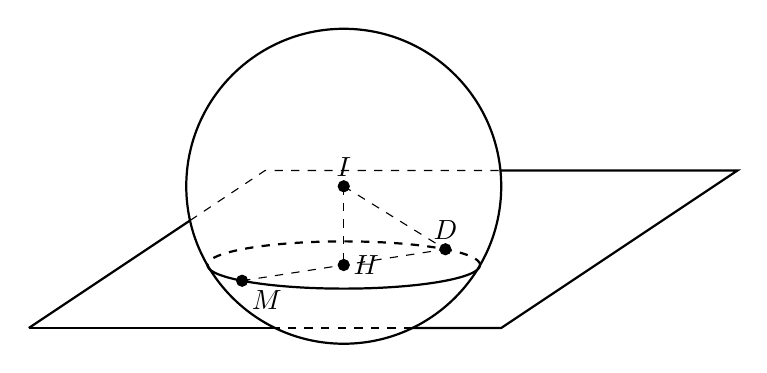
\begin{tikzpicture}
				\coordinate (P1) at (0,0);
				\coordinate (P2) at (2.04783,1.36522);
				\coordinate (P3) at (3,2);
				\coordinate (P4) at (5.989975,2);
				\coordinate (P5) at (9,2);
				\coordinate (P6) at (6,0);
				\coordinate (P7) at (4.871779,0);
				\coordinate (P8) at (3.12822,0);
				\coordinate (I) at (4,1.8);
				\coordinate (D) at (5.29099,1);
				\coordinate (H) at (4,0.8);
				\coordinate (M) at (2.709,0.6);
				\draw[thick] (P1) -- (P2);
				\draw[dashed] (P2) -- (P3) -- (P4);
				\draw[thick] (P4) -- (P5) -- (P6) -- (P7);
				\draw[dashed] (P7) -- (P8);
				\draw[thick] (P8) -- (P1);
				\draw[thick] (I) circle(2);
				\draw[dashed] (I) -- (H);
				\draw[dashed] (M) -- (D);
				\draw[dashed] (I) -- (D);
				\def\a{{sqrt(3)}}
				\def\b{0.3}
				\draw[dashed, thick] (5.732050807568878,0.8) arc[start angle=0, end angle=180, x radius=\a, y radius=\b];
				\draw[thick] (2.267949192431122,0.8) arc[start angle=180, end angle=360, x radius=\a, y radius=\b];
				\filldraw (I) circle(2pt) node[above] {$I$};
				\filldraw (D) circle(2pt) node[above] {$D$};
				\filldraw (H) circle(2pt) node[right] {$H$};
				\filldraw (M) circle(2pt) node[below right] {$M$};
			\end{tikzpicture}
		\end{center}
		Mặt cầu $(S) \colon (x+2)^2+(y-4)^2+z^2=39$ có tâm là $I(-2;4;0)$, bán kính $R=\sqrt{39}$.\\
		Gọi $M(x;y;z) \in (S)$. Ta có: $x^2+y^2+z^2=19-4x+8y$.\\
		$MA^2=(x-1)^2+y^2+z^2=20-6x+8y$.\\
		$\vec{MB}=(2-x;1-y;3-z)$; $\vec{MC}=(-x;2-y;-3-z)$.\\
		$\vec{MB} \cdot \vec{MC}=-2x+x^2+2-3y+y^2-9+z^2$$=19-4x+8y-2x-3y-7$ $=-6x+5y+12$.\\
		Suy ra $MA^2+2\vec{MB} \cdot \vec{MC}=-18x+18y+44$.\\
		Theo giả thiết $MA^2+2\vec{MB} \cdot \vec{MC}=8 \Leftrightarrow -18x+18y+44=8 \Leftrightarrow -x+y+2=0$.
		Do đó $M\in (P):-x+y+2=0$.\\
		Ta có $\mathrm{d}(I;(P))=\dfrac{\left| 8 \right|}{\sqrt{2}}=\sqrt{32}<\sqrt{39}$ nên mặt phẳng $(P)$ cắt mặt cầu $(S)$ theo giao tuyến là đường tròn $(C)$có bán kính $R_1$ với $R_1=\sqrt{R^2-d^2}=\sqrt{39-32}=\sqrt7$.\\
		Mặt khác ta có $\heva{&D,M \in (P)\\&D,M \in (S)} \Rightarrow D,M \in (C)$.\\
		Do đó độ dài $MD$ lớn nhất bằng $2R_1=2\sqrt{7}$.
	}
\end{ex}

%Câu 11
\begin{ex}%[2H3G1-4]
	Trong không gian tọa độ $Oxyz$, cho 5 điểm $A(1;0;0)$, $B(-1;1;0)$, $C(0;-1;0)$, $D(0;1;0)$, $E(0;3;0)$. $M$ là điểm thay đổi trên mặt cầu $(S) \colon x^2+(y-1)^2+z^2=1$. Giá trị lớn nhất của biểu thức $P=2\left| \vec{MA}+\vec{MB}+\vec{MC} \right|+3\left| \vec{MD}+\vec{ME} \right|$ là
	\choice
	{$12$}
	{\True $12\sqrt{2}$}
	{$24$}
	{$24\sqrt{2}$}
	\loigiai{
		Mặt cầu $(S)$ có tâm $I(0;1;0)$ bán kính $R=1$.\\
		Gọi trọng tâm tam giác $ABC$ là $G(0;0;0)$, trung điểm $DE$ là $N(0;2;0)$.\\
		do $G,N$ đều nằm trên $(S)$ và $I$ là trung điểm $GN$ nên $GN$ là đường kính của $(S)$.
		\begin{eqnarray*}
			&P&=2\left| \vec{MA}+\vec{MB}+\vec{MC} \right| +3\left|\vec{MD}+\vec{ME}\right|\\
			& &=2\left|3\vec{MG}\right| +3\left|\vec{MN}\right|\\
			& &=6MG+6MN=6(MG+MN)
		\end{eqnarray*}
		\begin{center}
			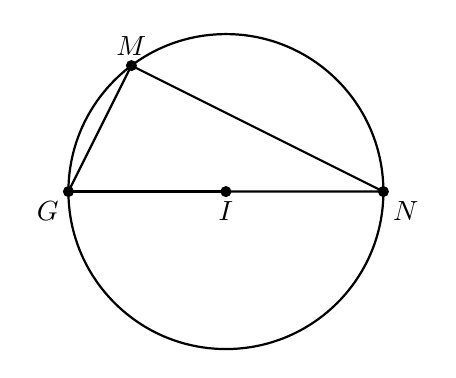
\begin{tikzpicture}
				\coordinate (G) at (-2, 0);
				\coordinate (I) at (0, 0);
				\coordinate (N) at (2, 0);
				\coordinate (M) at (-1.2, 1.6);
				\draw[thick] (I) circle (2);
				\draw[thick] (G) -- (M) -- (N) -- cycle;
				\draw[thick] (G) -- (I);
				\fill (G) circle (2pt);
				\fill (I) circle (2pt);
				\fill (N) circle (2pt);
				\fill (M) circle (2pt);
				\node[below left] at (G) {$G$};
				\node[below] at (I) {$I$};
				\node[below right] at (N) {$N$};
				\node[above] at (M) {$M$};
			\end{tikzpicture}
		\end{center}
		Ta có: $(MG+MN)^2\le 2(MG^2+MN^2)=2GN^2=8$.
		Suy ra $MG+MN\le 2\sqrt2$.\\
		Vậy giá trị lớn nhất của $P$ là $12\sqrt2$.
	}
\end{ex}

%Câu 12
\begin{ex}%[2H3G1-4]
	Trong không gian với hệ trục $Oxyz$, cho mặt cầu $(S) \colon (x+1)^2+(y-4)^2+z^2=8$ và điểm $A(3;0;0);B(4;2;1)$. Điểm $M$ thay đổi nằm trên mặt cầu, tìm giá trị nhỏ nhất của biểu thức $P=MA+2MB$.
	\choice
	{$P=2\sqrt{2}$}
	{$P=3\sqrt{2}$}
	{$P=4\sqrt{2}$}
	{\True $P=6\sqrt{2}$}
	\loigiai{
		\begin{center}
			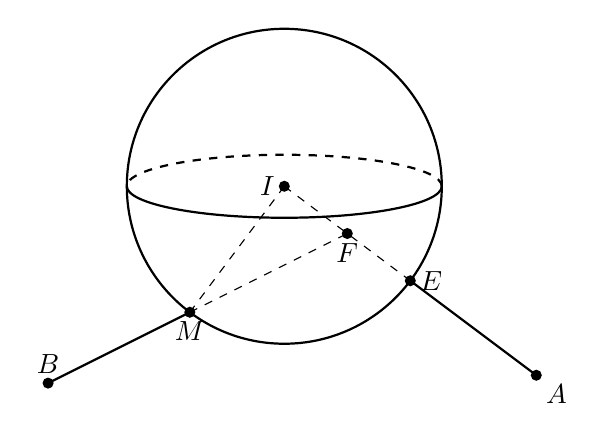
\begin{tikzpicture}
				\coordinate (E) at (1.6, -1.2);
				\coordinate (I) at (0, 0);
				\coordinate (A) at (3.2, -2.4);
				\coordinate (M) at (-1.2, -1.6);
				\coordinate (B) at (-3, -2.5);
				\coordinate (F) at (0.8, -0.6);
				\draw[thick] (I) circle (2);
				\draw[thick] (A) -- (E);
				\draw[dashed] (I) -- (E);
				\draw[thick] (M) -- (B);
				\draw[dashed] (M) -- (F);
				\draw[dashed] (I) -- (M);
				\def\a{2}
				\def\b{0.4}
				\draw[dashed, thick] (2,0) arc[start angle=0, end angle=180, x radius=\a, y radius=\b];
				\draw[thick] (-2,0) arc[start angle=180, end angle=360, x radius=\a, y radius=\b];
				\fill (E) circle (2pt);
				\fill (I) circle (2pt);
				\fill (A) circle (2pt);
				\fill (M) circle (2pt);
				\fill (B) circle (2pt);
				\fill (F) circle (2pt);
				\node[right] at (E) {$E$};
				\node[left] at (I) {$I$};
				\node[below right] at (A) {$A$};
				\node[below] at (M) {$M$};
				\node[above] at (B) {$B$};
				\node[below] at (F) {$F$};
			\end{tikzpicture}
		\end{center}
		Nhận xét: điểm $A,B$ nằm ngoài mặt cầu $(S)$. Mặt cầu $(S)$ có tâm $I(-1;4;0),R=2\sqrt2$.\\
		Ta có: $IA=4\sqrt2=2R,E=IA\cap (S)\Rightarrow E(1;2;0)$.\\
		Gọi $F$ là trung điểm của $IE\Rightarrow F(0;3;0)$.
		Tam giác $IFM$ và $IMA$ có $\widehat{AIM}$ chung và $\dfrac{IF}{IM}=\dfrac{1}{2}=\dfrac{IM}{IA} \Rightarrow \Delta AIM \sim \Delta MIF$.\\
		Suy ra $\dfrac{MA}{FM}=\dfrac{AI}{MI}=2\Rightarrow MA=2MF$.\\
		Ta có: $MA+2MB=2(MF+MB)\ge 2FB=6\sqrt2$.\\
		Vì $F$ nằm trong $(S)$ và $B$ nằm ngoài $(S)$ nên dấu $''=''$ xảy ra khi $M=BF \cap (S)$.\\
		Vậy giá trị nhỏ nhất là $P=6\sqrt{2}$.
	}
\end{ex}

%Câu 13 trùng 12
\begin{ex}%[2H3G1-4]
	Trong không gian với hệ trục $Oxyz$, cho mặt cầu $(S) \colon (x+1)^2+(y-4)^2+z^2=8$ và điểm $A(3;0;0)$, $B(4;2;1)$. Điểm $M$ thay đổi nằm trên mặt cầu, tìm giá trị nhỏ nhất của biểu thức $P=MA+2MB$.
	\choice
	{$P=2\sqrt{2}$}
	{$P=3\sqrt{2}$}
	{$P=4\sqrt{2}$}
	{\True $P=6\sqrt{2}$}
	\loigiai{
		Giả sử $M(x;y;z)$.
		Ta có: $\vec{AM}=(x-3;y;z)$, $\vec{BM}=(x-4;y-2;z-1)$.\\ Và $(x+1)^2+(y-4)^2+z^2=8$$\Leftrightarrow 3\left[ (x+1)^2+(y-4)^2+z^2-8 \right]=0$.\\
		Ta có:
		\begin{eqnarray*}
			&P&=MA+2MB\\
			&P&=\sqrt{(x-3)^2+y^2+z^2}+2\sqrt{(x-4)^2+(y-2)^2+(z-1)^2}\\
			&P&=\sqrt{(x-3)^2+y^2+z^2}+3\left[ (x+1)^2+(y-4)^2+z^2-8 \right]+2\sqrt{(x-4)^2+(y-2)^2+(z-1)^2}\\
			&P&=\sqrt{4x^2+4y^2-24y+4z^2+36}+2\sqrt{(x-4)^2+(y-2)^2+(z-1)^2}\\
			&P&=2\left[ \sqrt{x^2+(y-3)^2+z^2}+\sqrt{(x-4)^2+(y-2)^2+(z-1)^2} \right]\\
			&P&=2\left[ \sqrt{x^2+(y-3)^2+z^2}+\sqrt{(4-x)^2+(2-y)^2+(1-z)^2} \right]
		\end{eqnarray*}
		Áp dụng bất đẳng thức Minkowxki:\\
		$\sqrt{a^2+b^2+c^2}+\sqrt{d^2+e^2+f^2} \ge \sqrt{(a+d)^2+(b+e)^2+(c+f)^2}$.\\
		Dấu bằng xảy ra khi: $\dfrac{a}{d}=\dfrac{b}{e}=\dfrac{a}{f}>0$.\\
		$\Rightarrow P \ge 2\sqrt{(x+4-x)^2+(y-3+2-y)^2+(z+1-z)^2}=2\sqrt{4^2+(-1)^2+(1)^2}=6\sqrt{2}$.\\
		Dấu bằng xảy ra khi: $\heva{&\dfrac{4}{4-x}=\dfrac{y-3}{2-y}=\dfrac{z}{1-z}=t>0\\&(x+1)^2+(y-4)^2+z^2=8}$\\$ \Leftrightarrow \heva{&x=\dfrac{4t}{t+1}\\&y=\dfrac{2t+3}{t+1}\\&z=\dfrac{t}{t+1}\\& \left(\dfrac{5t+1}{t+1}\right)^2+ \left(\dfrac{-2t-1}{t+1}\right)^2+ \left(\dfrac{t}{t+1}\right)^2=8} \Leftrightarrow \heva{&x=\dfrac{4t}{t+1}\\&y=\dfrac{2t+3}{t+1}\\&z=\dfrac{t}{t+1}\\&22t^2-2t-6=0}$\\$ \Leftrightarrow \heva{&x=\dfrac{4+4\sqrt{133}}{23+\sqrt{133}}\\&y=\dfrac{34+\sqrt{133}}{23+\sqrt{133}}\\&z=\dfrac{1+\sqrt{133}}{23+\sqrt{133}}\\&t=\dfrac{1+\sqrt{133}}{22}}$\\
		Vậy giá trị nhỏ nhất của biểu thức là $6\sqrt{2}$.
	}
\end{ex}

%Câu 14
\begin{ex}%[2H3G1-4]
	Trong KG $Oxyz$, cho mặt cầu $(S) \colon (x-1)^2+y^2+(z-2)^2=10$ và hai điểm $A(1;2;-4)$ và $B(1;2;14)$. Điểm $M$ thay đổi trên mặt cầu $(S)$. Giá trị nhỏ nhất của $(MA+2MB)$ bằng
	\choice
	{$2\sqrt{82}$}
	{$3\sqrt{79}$}
	{$5\sqrt{79}$}
	{\True $3\sqrt{82}$}
	\loigiai{
		$(S)$ có tâm $I(1;0;2)$ và bán kính $R=\sqrt10$.\\
		Ta có $IA=2\sqrt10=2R$ nên tồn tại điểm $C$ cố định sao cho $MA=2MC$ $\forall M\in (S)$ $(1)$.\\
		Thật vậy, gọi $(a;b;c)$ là tọa độ điểm $C$. Khi đó, với mọi điểm $M(x;y;z)\in (S) \\ \Rightarrow x^2+y^2+z^2=2x+4z+5$, ta có:\\
		$\bullet MA^2=(x-1)^2+(y-2)^2+(z+4)^2=x^2+y^2+z^2-2x-4y+8z+21$\\
		$=2x+4z+5-2x-4y+8z+21=-4y+12z+26$\\
		$\bullet MC^2=(x-a)^2+(y-b)^2+(z-c)^2=x^2+y^2+z^2-2ax-2by-2cz+a^2+b^2+c^2$.\\
		$=2x+4z+5-2ax-2by-2cz+a^2+b^2+c^2=(2-2a)x-2by+(4-2c)z+a^2+b^2+c^2+5$.\\
		Nên $(1)\Leftrightarrow MA^2=4MC^2$ $\forall M\in (S)$\\
		$\Leftrightarrow -4y+12z+26=4\left[ (2-2a)x-2by+(4-2c)z+a^2+b^2+c^2+5 \right], \forall x,y,z$\\ $\heva{&4(2-2a)=0\\&4(-2b)\-4\\&4(4-2c)=12\\&4(a^2+b^2+c^2+5)=26} \Leftrightarrow \heva{&a=1\\&b=\dfrac{1}{2}\\&c=\dfrac{1}{2}} \Rightarrow C\left(1;\dfrac{1}{2};\dfrac{1}{2}\right)$.\\
		Lúc này, $IC=\dfrac{\sqrt{10}}{2}<R<IB=2\sqrt{37}$ nên $C$ nằm trong $(S)$ còn $B$ nằm ngoài $(S)$ và \\
		$MA+2MB=2MC+2MB=2(MC+MB)\ge 2BC=3\sqrt{82}$.\\
		Đẳng thức xảy ra $\Leftrightarrow M$ là giao điểm của đoạn $BC$ và mặt cầu $(S)$.\\
		Vậy $\min (MA+2MB)=3\sqrt{82}$.
	}
\end{ex}

%Câu 15
\begin{ex}%[2H3G1-4]
	Trong KG $Oxyz$, cho hai điểm $A(-1;0;0)$ và $B(2;3;4)$. Gọi $(P)$ là mặt phẳng chứa đường tròn giao tuyến của hai mặt cầu $(S_1) \colon (x-1)^2+(y+1)^2+z^2=4$ và $(S_2) \colon x^2+y^2+z^2+2y-2=0$. Xét $M$, $N$ là hai điểm bất kỳ thuộc mặt phẳng $(P)$ sao cho $MN=1$. Giá trị nhỏ nhất của $AM+BN$ bằng
	\choice
	{\True $5$}
	{$3$}
	{$6$}
	{$4$}
	\loigiai{
		\begin{center}
			\begin{tikzpicture}
				\coordinate (B) at (4.5,3);
				\coordinate (D) at (4.5,1.5);
				\coordinate (N) at (2.5,1.5);
				\coordinate (C) at (1.5,1);
				\coordinate (M) at (3.5,0.5);
				\coordinate (K) at (1.5,0);
				\coordinate (A) at (1.5,-1);
				\coordinate (M1) at (0,0);
				\coordinate (M2) at (1.5,2);
				\coordinate (M3) at (4.5,0);
				\coordinate (M4) at (6,2);
				\draw[thick] (M1) -- (M2) -- (M4) -- (M3) -- cycle;
				\draw[thick] (B) -- (D);
				\draw[thick] (N) -- (D);
				\draw[thick] (B) -- (N);
				\draw[thick] (N) -- (M);
				\draw[thick] (C) -- (D);
				\draw[thick] (C) -- (M);
				\draw[thick] (A) -- (M);
				\draw[thick] (A) -- (K);
				\draw[dashed] (K) -- (C);
				\filldraw (B) circle(2pt) node[above] {B};
				\filldraw (D) circle(2pt) node[right] {D};
				\filldraw (N) circle(2pt) node[left] {N};
				\filldraw (M) circle(2pt) node[right] {M};
				\filldraw (C) circle(2pt) node[left] {C};
				\filldraw (A) circle(1.5pt) node[below] {A};
				\pic[draw=blue, - , angle eccentricity=1.2, angle radius=1cm]
				{angle=M3--M1--M2};
			\end{tikzpicture}
		\end{center}
		Xét hệ $\heva{&(x-1)^2+(y+1)^2+z^2=4\\&x^2+y^2+z^2+2y-2=0} \Leftrightarrow \heva{&x^2+y^2+z^2-2x+2y-2=0\\&x^2+y^2+z^2+2y-2=0} \Rightarrow x=0$.\\
		Vậy $(P):x=0$ ((P) chính là mặt phẳng $(Oyz)$).\\
		Gọi $C(0;0;0)$ và $D(0;3;4)$ lần lượt là hình chiếu vuông góc của $A(-1;0;0)$ và $B(2;3;4)$trên mặt phẳng $(P)$. Suy ra $AC=1$, $BD=2$, $CD=5$.\\
		Áp dụng bất đẳng thức $\sqrt{a^2+b^2}+\sqrt{c^2+d^2}\ge \sqrt{(a+c)^2+(b+d)^2}$, ta được\\
		\begin{eqnarray*}
			&AM+BN&=\sqrt{AC^2+CM^2}+\sqrt{BD^2+DN^2}\\
			&&\ge \sqrt{(AC+BD)^2+(CM+DN)^2}\\
			&&\ge \sqrt{9+(CM+DN)^2}
		\end{eqnarray*}
		Lại có $CM+MN+ND\ge CD=5$ nên suy ra $CM+ND\ge 4$. Do đó $AM+BN\ge 5$.\\
		Đẳng thức xảy ra khi $C$, $M$, $N$, $D$ thẳng hàng theo thứ tự đó và $\dfrac{AC}{CM}=\dfrac{BD}{DN}$\\
		Tức là $M\left(0;\dfrac{4}{5};\dfrac{16}{15}\right)$ và $N\left(0;\dfrac{7}{5};\dfrac{28}{15}\right)$.\\
		Vậy giá trị nhỏ nhất của $AM+BN$ là $5$.
	}
\end{ex}

%Câu 16
\begin{ex}%[2H3G1-4]
	Trong KG $Oxyz$, cho các điểm $A(0;0;2)$ và $B(3;4;1)$. Gọi $(P)$ là mặt phẳng chứa đường tròn giao tuyến của hai mặt cầu $(S_1) \colon (x-1)^2+(y-1)^2+(z+3)^2=25$ với $(S_2) \colon x^2+y^2+z^2-2x-2y-14=0$. $M$, $N$ là hai điểm thuộc $(P)$ sao cho $MN=1$. Giá trị nhỏ nhất của $AM+BN$ là
	\choice
	{$\sqrt{34}-1$}
	{\True $5$}
	{$\sqrt{34}$}
	{$3$}
	\loigiai{
		\begin{center}
			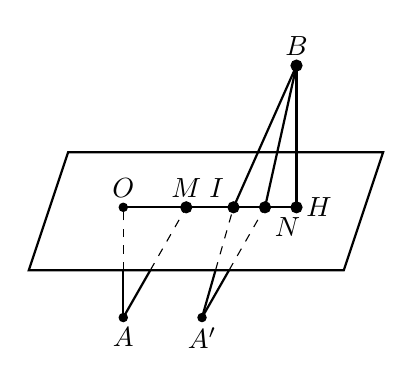
\begin{tikzpicture}
				\coordinate (B) at (3.4,2.6);
				\coordinate (H) at (3.4,0.8);
				\coordinate (N) at (3,0.8);
				\coordinate (I) at (2.6,0.8);
				\coordinate (M) at (2,0.8);
				\coordinate (O) at (1.2,0.8);
				\coordinate (A1) at (1.2,-0.6);
				\coordinate (A2) at (2.2,-0.6);
				\coordinate (T1) at (1.2,0);
				\coordinate (T2) at ({54/35},0);
				\coordinate (T3) at ({83/35},0);
				\coordinate (T4) at ({89/35},0);
				\coordinate (M1) at (0,0);
				\coordinate (M2) at (0.5,1.5);
				\coordinate (M3) at (4.5,1.5);
				\coordinate (M4) at (4,0);
				\draw[thick] (M1) -- (M2) -- (M3) -- (M4) -- cycle;
				\draw[thick] (B) -- (H);
				\draw[thick] (B) -- (N);
				\draw[thick] (B) -- (I);
				\draw[thick] (O) -- (H);
				\draw[thick] (A1) -- (T1);
				\draw[thick] (A1) -- (T2);
				\draw[thick] (A2) -- (T3);
				\draw[thick] (A2) -- (T4);
				\draw[dashed] (T1) -- (O);
				\draw[dashed] (T2) -- (M);
				\draw[dashed] (T3) -- (I);
				\draw[dashed] (T4) -- (N);
				\filldraw (B) circle(2pt) node[above] {$B$};
				\filldraw (H) circle(2pt) node[right] {$H$};
				\filldraw (N) circle(2pt) node[below right] {$N$};
				\filldraw (I) circle(2pt) node[above left] {$I$};
				\filldraw (M) circle(2pt) node[above] {$M$};
				\filldraw (O) circle(1.5pt) node[above] {$O$};
				\filldraw (A1) circle(1.5pt) node[below] {$A$};
				\filldraw (A2) circle(1.5pt) node[below] {$A'$};
			\end{tikzpicture}
		\end{center}
		Từ $\heva{&(S_1) \colon (x-1)^2+(y-1)^2+(z+3)^2=25 (1)\\&(S_2) \colon x^2+y^2+z^2-2x-2y-14=0 (2)}$\\
		Lấy $(1)$ trừ $(2)$, ta được $6z=0$ hay $(P) \colon z=0 \Rightarrow (P) \equiv (Oxy)$.\\
		Dễ thấy $A$, $B$ nằm khác phía đối với $(P)$, hình chiếu của $A$ trên $(P)$ là $O$, hình chiếu của $B$ trên $(P)$ là $H(3;4;0).$\\
		Lấy $A'$ sao cho $\vec{AA'}=\vec{MN}$.\\
		Khi đó $AM+BN=A'N+BN \ge A'B$ và cực trị chỉ xảy ra khi $\vec{MN}$ cùng phương $\vec{OH}$.\\
		Lấy $\vec{MN}=\dfrac{\vec{OH}}{\left| \vec{OH} \right|}=\left(\dfrac{3}{5};\dfrac{4}{5};0\right)$.\\
		Khi đó vì $\vec{AA'}=\vec{MN}$ nên $A'\left(\dfrac{3}{5};\dfrac{4}{5};0\right)$. Do đó $AM+BN=A'N+BN\ge A'B=5$.
	}
\end{ex}

%Câu 17
\begin{ex}%[2H3G1-4]
	Trong KG $Oxyz$ cho mặt cầu $(S)$ có phương trình $x^2+y^2+z^2-4x+2y-2z-3=0$ và điểm $A(5;3;-2)$. Một đường thẳng $d$ thay đổi luôn đi qua $A$ và luôn cắt mặt cầu tại hai điểm phân biệt $M,N$. Tính giá trị nhỏ nhất của biểu thức $S=AM+4AN$.
	\choice
	{$S_{\min} =30$}
	{$S_{\min} =20$}
	{$S_{\min} =\sqrt{34}-3$}
	{\True $S_{\min} =5\sqrt{34}-9$}
	\loigiai{
		Mặt cầu $(S)$ có tâm $I(2;-1;1)$, bán kính $R=3$.\\
		$AI=\sqrt{34}>R \Rightarrow A$ nằm ngoài mặt cầu $(S)$.\\
		\begin{center}
			\begin{tikzpicture}
				\coordinate (M) at ({sqrt(2.3)},{sqrt(1.7)});
				\coordinate (N) at (-{sqrt(3.687286253)},{sqrt(0.3127147469)});
				\coordinate (A) at (-4.5,0);
				\coordinate (I) at (0,0);
				\coordinate (H) at ($(N)!0.5!(M)$);
				\draw[thick] (I) circle (2);
				\draw[thick] (I) -- (A) -- (H) -- cycle;
				\draw[thick] (H) -- (M);
				\filldraw (M) circle(2pt) node[right] {$M$};
				\filldraw (H) circle(2pt) node[above] {$H$};
				\filldraw (N) circle(2pt) node[above left] {$N$};
				\filldraw (A) circle(2pt) node[left] {$A$};
				\filldraw (I) circle(2pt) node[below right] {$I$};
			\end{tikzpicture}
		\end{center}
		Do hai điểm $M,N$ nằm ở vị trí hai đầu một dây cung nên để $S_{\min}$ thì $N$ nằm giữa $A$ và $M$. Gọi $H$ là trung điểm $MN \Rightarrow IH \bot MN, NH=\dfrac{1}{2}MN$.\\ 
		$S=4(AH-NH)+AH+NH=5AH-3NH$\\
		$S=5\sqrt{AI^2-IH^2}-3\sqrt{R^2-IH^2}=5\sqrt{34-x^2}-3\sqrt{9-x^2}, x=IH$\\
		Xét hàm số $f(x)=5\sqrt{34-x^2}-3\sqrt{9-x^2}, (0 \le x < 3)$\\
		$f'(x)=\dfrac{-5x}{\sqrt{34-x^2}}+\dfrac{3x}{\sqrt{9-x^2}}=x \left(\dfrac{-5}{\sqrt{34-x^2}}+\dfrac{3}{\sqrt{9-x^2}}\right)$\\
		Xét $\left(\dfrac{-5}{\sqrt{34-x^2}}+\dfrac{3}{\sqrt{9-x^2}}\right)>0$\\
		$\Leftrightarrow 5\sqrt{9-x^2}<3\sqrt{34-x^2} \Leftrightarrow 225-25x^2<9 \cdot 34-9x^2 \Leftrightarrow 16x^2+81>0$ (luôn đúng).\\
		Suy ra $f'(x) \ge 0, \forall x \in [0;3), f'(x)=0 \Leftrightarrow x=0 \Rightarrow f(x)$ đồng biến trên $[0;3)$\\
		Suy ra $\underset{ [0;3) }{\mathop{\min }}\, f(x)=f(0)=5\sqrt{34}-9$.
	}
\end{ex}

%Câu 18
\begin{ex}%[2H3G1-4]
	Trong KG $Oxyz$ cho đường thẳng $d \colon \dfrac{x-1}{2}=\dfrac{y-2}{3}=\dfrac{z-3}{4}$ và mặt cầu $(S) \colon (x+3)^2+(y+4)^2+(z+5)^2=729$. Cho biết điểm $A(-2;-2;-7)$, điểm $B$ thuộc giao tuyến của mặt cầu $(S)$ và mặt phẳng $(P) \colon 2x+3y+4z-107=0$. Khi điểm $M$ di động trên đường thẳng $d$ giá trị nhỏ nhất của biểu thức $MA+MB$ bằng
	\choice
	{\True $5\sqrt{30}$}
	{$27$}
	{$5\sqrt{29}$}
	{$\sqrt{742}$}
	\loigiai{
		\begin{center}
			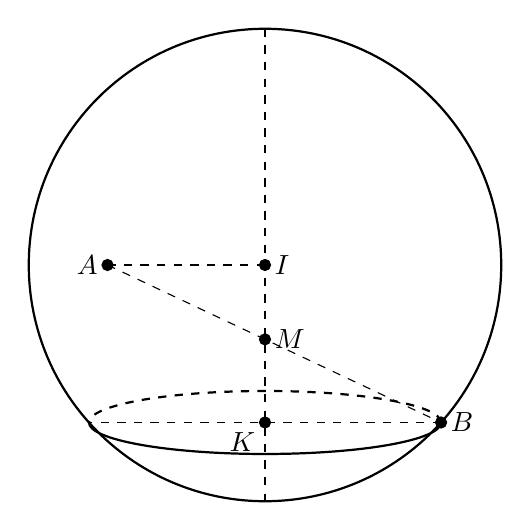
\begin{tikzpicture}
				\coordinate (P1) at (0,3);
				\coordinate (I) at (0,0);
				\coordinate (A) at (-2,0);
				\coordinate (M) at (0,-0.9442719);
				\coordinate (B) at (2.236068,-2);
				\coordinate (K) at (0,-2);
				\coordinate (P2) at (-2.236068,-2);
				\coordinate (P3) at (0,-3);
				\draw[thick] (I) circle(3);
				\draw[dashed] (P1) -- (P3);
				\draw[dashed] (I) -- (A);
				\draw[dashed] (A) -- (B);
				\draw[dashed] (B) -- (P2);
				\def\a{2.2360678}
				\def\b{0.4}
				\draw[dashed, thick] (2.236068,-2) arc[start angle=0, end angle=180, x radius=\a, y radius=\b];
				\draw[thick] (-2.236068,-2) arc[start angle=180, end angle=360, x radius=\a, y radius=\b];
				\filldraw (I) circle(2pt) node[right] {$I$};
				\filldraw (A) circle(2pt) node[left] {$A$};
				\filldraw (M) circle(2pt) node[right] {$M$};
				\filldraw (B) circle(2pt) node[right] {$B$};
				\filldraw (K) circle(2pt) node[below left] {$K$};
			\end{tikzpicture}
		\end{center}
		Mặt cầu $(S)$ có tâm $I(-3;-4;-5)$ và bán kính $R=27$.\\
		Đường thẳng $d$ có 1 véc-tơ chỉ phương là $\vec{u}=(2;3;4)\Rightarrow d\bot(P)$.\\
		Gọi $K$ là giao điểm của mặt phẳng $(P)$ và đường thẳng $d$. Vì $I\in d$ nên $K$ là tâm của đường tròn giao tuyến và $KB\bot d$.\\
		Ta có $\vec{IA}=(1;2;-2)\Rightarrow IA=3$ và $\vec{IA}.\vec{u}=0\Rightarrow IA\bot d$.\\
		Ta tính được $IK=\text{d(I,(P))}=\dfrac{\left| 2 \cdot (-3)+3 \cdot (-4)+4(-5)-107 \right|}{\sqrt{2^2+3^2+4^2}}=5\sqrt{29}$\\ Và $KB=\sqrt{R^2-IK^2}=2$.\\
		Do $M$ di động trên đường thẳng $d$ (trục của đường tròn giao tuyến) và $B$ thuộc đường tròn giao tuyến nên biểu thức $MA+MB$ nhỏ nhất khi và chỉ khi $M=AB\cap d$.\\
		Khi đó, ta có $\dfrac{MI}{MK}=\dfrac{IA}{KB}=\dfrac{3}{2}$ và $MI+MK=IK=5\sqrt{29}$.\\
		Suy ra $MI=3\sqrt{29}$, $MK=2\sqrt{29}$.\\
		Ta có $AM=\sqrt{IA^2+MI^2}=3\sqrt{30}\Rightarrow BM=\dfrac{2}{3}AM=2\sqrt{30}$.\\
		Vậy giá trị nhỏ nhất của $MA+MB$ là $AM+BM=3\sqrt{30}+2\sqrt{30}=5\sqrt{30}$.\\
		Cách 2:
		Ta có $(S)$ có tâm $I(-3;-4;-5)$, bán kính $R=27$.\\
		Dễ thấy $d$ đi qua $I(-3;-4;-5)$và vuông góc với $(P)$.\\
		$(P)$ cắt $(S)$ theo đường tròn có bán kính $r=2$.
		$M\in d\Leftrightarrow M(1+2t;2+3t;3+4t)$.\\
		Ta có $T=MA+MB=MA+\sqrt{MH^2+r^2}$.\\
		Lại có $MH=d(M;(P))=\dfrac{\left| 29t-87 \right|}{\sqrt{29}}=\left| \sqrt{29}t-3\sqrt{29}\right|$.\\
		Suy ra\\ $T=\sqrt{29t^2+116t+125}+\sqrt{29(t-3)^2+4}$\\
		$T=\sqrt{29}\sqrt{(t+2)^2+\dfrac{9}{29}}+\sqrt{29}\sqrt{(t-3)^2+\dfrac{4}{29}}$.\\
		Xét $\vec{u}=\left(t+2;\dfrac{3}{\sqrt{29}}\right)$, $\vec{v}=\left(3-t;\dfrac{2}{\sqrt{29}}\right)\Rightarrow \vec{u}+\vec{v}=\left(5;\dfrac{5}{\sqrt{29}}\right)$.\\
		Do đó $T=\sqrt{29}(\left| \vec{u} \right|+\left| \vec{v} \right|) \ge \sqrt{29}\left| \vec{u}+\vec{v} \right|=5\sqrt{50}$.
	}
\end{ex}

%Câu 19
\begin{ex}%[2H3G1-4]
	Trong không gian với hệ trục tọa độ $Oxyz$, cho hai mặt cầu $(S_1) \colon x^2+y^2+z^2=1$, $(S_2) \colon x^2+(y-4)^2+z^2=4$ và các điểm $A(4;0;0)$, $B\left(\dfrac{1}{4};0;0\right)$, $C(1;4;0)$, $D(4;4;0)$. Gọi $M$ là điểm thay đổi trên $(S_1)$, $N$ là điểm thay đổi trên $(S_2)$. Giá trị nhỏ nhất của biểu thức $Q=MA+2ND+4MN+4BC$ là
	\choice
	{\True $2\sqrt{265}$}
	{$\sqrt{265}$}
	{$3\sqrt{265}$}
	{$4\sqrt{265}$}
	\loigiai{
		\begin{center}
			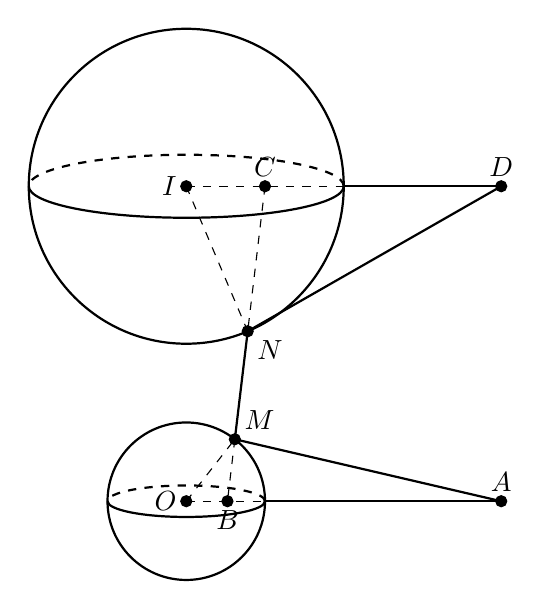
\begin{tikzpicture}
				\coordinate (I) at (0,4);
				\coordinate (C) at (1,4);
				\coordinate (D) at (4,4);
				\coordinate (N) at (0.78041,2.158544);
				\coordinate (M) at (0.616865765,0.7870683);
				\coordinate (O) at (0,0);
				\coordinate (B) at (0.523,0);
				\coordinate (A) at (4,0);
				\coordinate (P1) at (2,4);
				\coordinate (P2) at (1,0);
				\draw [thick] (O) circle(1);
				\draw [thick] (I) circle(2);
				\draw [dashed] (I) -- (P1);
				\draw [dashed] (I) -- (N);
				\draw [dashed] (C) -- (N);
				\draw [dashed] (O) -- (M);
				\draw [dashed] (O) -- (P2);
				\draw [dashed] (M) -- (B);
				\draw [thick] (P1) -- (D);
				\draw [thick] (N) -- (D);
				\draw [thick] (N) -- (M);
				\draw [thick] (M) -- (A);
				\draw [thick] (P2) -- (A);
				\draw[dashed, thick] (2,4) arc[start angle=0, end angle=180, x radius=2, y radius=0.4];
				\draw[thick] (-2,4) arc[start angle=180, end angle=360, x radius=2, y radius=0.4];
				\draw[dashed, thick] (1,0) arc[start angle=0, end angle=180, x radius=1, y radius=0.2];
				\draw[thick] (-1,0) arc[start angle=180, end angle=360, x radius=1, y radius=0.2];
				\filldraw (I) circle(2pt) node[left] {$I$};
				\filldraw (C) circle(2pt) node[above] {$C$};
				\filldraw (D) circle(2pt) node[above] {$D$};
				\filldraw (N) circle(2pt) node[below right] {$N$};
				\filldraw (M) circle(2pt) node[above right] {$M$};
				\filldraw (O) circle(2pt) node[left] {$O$};
				\filldraw (B) circle(2pt) node[below] {$B$};
				\filldraw (A) circle(2pt) node[above] {$A$};
			\end{tikzpicture}
		\end{center}
		$(S_1): x^2 + y^2 + z^2 = 1$ nên $(S_1)$ có tâm $O(0;0;0)$ và bán kính $R_1 = 1$.\\
		$(S_2): x^2 + (y-4)^2 + z^2 = 4$ nên $(S_2)$ có tâm $I(0;4;0)$ và bán kính $R_2 = 2$.\\
		Vậy các điểm $A(4;0;0)$, $B\left(\dfrac{1}{4};0;0\right)$, $C(1;4;0)$, $D(4;4;0)$, $O(0;0;0)$ và $I(0;4;0)$ cùng thuộc $(Oxy)$.\\
		Nhận thấy $OB \cdot OA = OM^2$ suy ra $OM$ là tiếp tuyến của đường tròn ngoại tiếp tam giác $MAB$.\\
		Do đó $\Delta MOB$ đồng dạng $\Delta AOM$.\\
		$\Rightarrow \dfrac{MA}{MB} = \dfrac{OA}{OM} = 4 \Rightarrow MA = 4MB$.\\
		Hoàn toàn tương tự $\dfrac{ND}{NC} = \dfrac{DI}{NI} = 2 \Rightarrow ND = 2NC$.\\
		Xét:\\
		$Q = MA + 2ND + 4MN + 4BC$\\
		$Q = 4(MB + NC + MN) + 4BC \ge 4BC + 4BC = 8BC = 2\sqrt{265}$.
	}
\end{ex}
\begin{ex}%[2H5C3-2]
	Trong KG $Oxyz$, cho mặt cầu $(S)\colon x^2+y^2+z^2-2x-4y-4=0$ và hai điểm $A(4;2;4)$, $B(1;4;2)$. $MN$ là dây cung của mặt cầu thỏa mãn $\overrightarrow{MN}$ cùng hướng với $\overrightarrow{u}=(0;1;1)$ và $MN=4\sqrt{2}$. Tính giá trị lớn nhất của $\left|AM-BN\right|$.
	\choice
	{$\sqrt{41}$}
	{$4\sqrt{2}$}
	{\True $7$}
	{$\sqrt{17}$}
	\loigiai{
		\begin{center}
			\begin{tikzpicture}[scale=0.75, font=\footnotesize, line join=round, line cap=round, >=stealth]
				\def\R{2} % Bán kính
				\coordinate (I) at (0,0);
				\coordinate (x) at (\R,0);
				\draw[name path=DTO](I) circle (\R) (x) arc (0:-180: {\R} and {\R/2});
				\draw[dashed] (x) arc (0:180: {\R} and {\R/2});
				\coordinate (M) at ($({\R*cos(-30)},{\R*sin(-30)})$);
				\coordinate (N) at ($({\R*cos(-85)},{\R*sin(-85)})$);
				\coordinate (M') at ($({\R*cos(100)},{\R*sin(100)})$);
				\coordinate (N') at ($({\R*cos(155)},{\R*sin(155)})$);
				\coordinate (B) at ($(N)!0.25!(N')$);
				\coordinate (A') at ($(N)!3/2!(N')$);
				\coordinate (A) at ($(M)!3/2!(M')$);
				\path[name path=AI] (A)--(I);
				\path[name path=AB] (A)--(B);
				\path[name intersections={of= AI and DTO,by={I'}}];
				\path[name intersections={of= AB and DTO,by={B'}}];
				\draw[dashed](M')--(M)--(N)--(N')(A)--(I)--(B)--(M)--(I)(B)--(B');
				\draw(M')--(A)--(A')--(N')(A)--(B');
				\foreach \x/\g in {I/20,M/0,N/-90,B/-120,A'/-120,A/90} \fill[black](\x)circle(1pt) +(\g:.4)node[scale=1]{$\x$};
			\end{tikzpicture}
		\end{center}
		Tâm $I(1;2;0)$, bán kính $R=3$.\\
		Ta có $\overrightarrow{IA}=(3;0;4)\Rightarrow IA=5$, $\overrightarrow{IB}=(0;2;2)\Rightarrow IB=2\sqrt{2}$ nên điểm $A(4;2;4)$nằm ngoài mặt cầu $(S)$ và điểm $B(1;4;2)$ nằm trong mặt cầu $(S)$.\\
		Do $\overrightarrow{MN}$ cùng hướng với $\overrightarrow{u}=(0;1;1)$ suy ra $\overrightarrow{MN}=\left( 0;k;k \right),\,k>0$ do $MN=4\sqrt{2}$ suy ra $\overrightarrow{MN}=\left( 0;4;4 \right)$.\\
		Gọi $A'={T_{\overrightarrow{MN}}}(A)$, suy ra $A'=(4;6;8)$.\\
		Khi đó $AMNA'$ là hình bình hành nên $AM=A'N$\\
		Ta có $\left|AM-BN\right|=\left|A'N-BN\right|\le A'B$.\\
		Dấu \lq\lq=\rq\rq xảy ra khi $A'$, $N$, $B$ thẳng hàng $\Leftrightarrow N$ là giao điểm của mặt cầu với đường thẳng $A'B$. (Điểm $N$ luôn tồn tại).\\
		$\overrightarrow{A'B}=(-3;-2;-6)$ suy ra $A'B=\sqrt{(-3)^2+(-2)^2+(-6)^2}=7$.\\
		Vậy ${{\left|AM-BN\right|}_{\min}}=A'B=7$.}
\end{ex}
\begin{ex}%[2H5C3-3]
	Trong KG $Oxyz$, gọi điểm $M(a;b;c)$ (với $a$, $b$, $c$ là các phân số tối giản) thuộc mặt cầu $(S)\colon x^2+y^2+z^2-2x-4y-4z-7=0$ sao cho biểu thức $T=2a+3b+6c$ đạt giá trị lớn nhất. Khi đó giá trị biểu thức $P=2a-b+c$ bằng
	\choice
	{$\dfrac{12}{7}$}
	{$8$}
	{\True $6$}
	{$\dfrac{51}{7}$}
	\loigiai{
		$x^2+y^2+z^2-2x-4y-4z-7=0\Leftrightarrow (x-1)^2+(y-2)^2+(z-2)^2=16$.\\
		$M(a;b;c)\in (S)\Leftrightarrow (a-1)^2+(b-2)^2+(c-2)^2=16$.\\
		Ta có $\left| 2(a-1)+3(b-2)+6(c-2) \right|\le \sqrt{\left( {2^2}+3^2+6^2 \right)\cdot \left[ (a-1)^2+(b-2)^2+(c-2)^2 \right]}$.\\
		$\Leftrightarrow \left| 2a+3b+6c-20 \right|\le 28\Rightarrow 2a+3b+6c-20\le 28\Rightarrow 2a+3b+6c\le 48$.\\
		Dấu \lq\lq=\rq\rq xảy ra khi
		$\heva{&2a+3b+6c=48\\&\dfrac{a-1}{2}=\dfrac{b-2}{3}\\&\dfrac{a-1}{2}=\dfrac{c-2}{6}}\Leftrightarrow\heva{&2a+3b+6c=48\\&3a-2b=-1\\&3a-c=1}\Leftrightarrow\heva{&a=\dfrac{15}{7}\\&b=\dfrac{26}{7}\\&c=\dfrac{38}{7}.}$\\
		Vậy $P=2a-b+c=2\cdot\dfrac{15}{7}-\dfrac{26}{7}+\dfrac{38}{7}=6$.}
\end{ex}
\begin{ex}%[2H5C3-3]
	Cho $x$, $y$, $z$, $a$, $b$, $c$ là các số thực thay đổi thỏa mãn $(x+1)^2+(y+1)^2+(z-2)^2=1$ và $a+b+c=3.$ Tìm giá trị nhỏ nhất của $P=(x-a)^2+(y-b)^2+(z-c)^2$.
	\choice
	{$\sqrt{3}-1$}
	{$\sqrt{3}+1$}
	{\True $4-2\sqrt{3}$}
	{$4+2\sqrt{3}$}
	\loigiai{
		\immini{Gọi $M(x;y;z)\Rightarrow M$ thuộc mặt cầu $(S)$tâm $I(-1;-1;2)$ bán kính $R=1$.\\
			Gọi $H(a;b;c)\Rightarrow H$ thuộc mặt phẳng $(P)\colon x+y+z-3=0$\\
			Ta có $\mathrm{d}(I,(P))=\dfrac{\left| -1-1+2-3 \right|}{\sqrt{3}}=\sqrt{3}>R\Rightarrow (P)$và $(S)$ không có điểm chung.\\
			$P=(x-a)^2+(y-b)^2+(z-c)^2=MH^2$ đạt giá trị nhỏ nhất khi vị trí của $M$ và $H$ như hình vẽ\\
			Khi đó $HI=\mathrm{d}(I,(P))=\sqrt{3}\Rightarrow HM=HI-R=\sqrt{3}-1$\\
			Do đó ${P_{\min }}={{\left( \sqrt{3}-1 \right)}^2}=4-2\sqrt{3}$.}
		{\begin{tikzpicture}[scale=0.75, font=\footnotesize, line join=round, line cap=round, >=stealth]
				\def\R{2.5} % Bán kính
				\coordinate (I) at (0,0);
				\coordinate (M) at (0,-\R);
				\coordinate (H) at (0,-2*\R);
				\coordinate (A) at (-4,-6);
				\coordinate (B) at (-3,-4);
				\coordinate (C) at (2,-6);
				\draw (-4,-6)--(-3,-4)--(3,-4)--(2,-6)--(-4,-6);
				\draw[dashed](I)--(H);
				\coordinate[label=below right:$(P)$] (P) at (-3.9,-5.3);
				\coordinate[label=below right:$(S)$] (S) at (2,2);
				\draw(I) circle (\R);
				\draw pic[angle eccentricity=2.2,draw,angle radius=25]{angle=C--A--B};
				\foreach \y/\g in {I/90,M/-40,H/0}
				\fill[black] (\y) circle(1.5pt) ($(\y)+(\g:3.5mm)$) node{$\y$};
		\end{tikzpicture}}
	}
\end{ex}
\begin{ex}%[2H5C3-3]
	Trong KG $Oxyz$, cho hai điểm $A(-2;2;-2)$; $B(3;-3;3)$. Điểm $M$ trong không gian thỏa mãn $\dfrac{MA}{MB}=\dfrac{2}{3}$. Khi đó độ dài $OM$ lớn nhất bằng
	\choice
	{$6\sqrt{3}$}
	{\True $12\sqrt{3}$}
	{$\dfrac{5\sqrt{3}}{2}$}
	{$5\sqrt{3}$}
	\loigiai{
		Gọi $M(x;y;z)$. Ta có\\
		\begin{eqnarray*}
			\dfrac{MA}{MB}=\dfrac{2}{3}
			&\Leftrightarrow & 9MA^2=4MB^2\\
			&\Leftrightarrow & 9\left[ (x+2)^2+(y-2)^2+(z+2)^2 \right]=4\left[ (x-3)^2+(y+3)^2+(z-3)^2 \right]\\
			&\Leftrightarrow & x^2+y^2+z^2+12x-12y+12z=0\\
			&\Leftrightarrow & (x+6)^2+(y-6)^2+(z+6)^2=108.
		\end{eqnarray*}
		Như vậy, điểm $M$ thuộc mặt cầu $(S)$ tâm $I(-6;6;-6)$ và bán kính $R=\sqrt{108}=6\sqrt{3}$.\\
		Do đó $OM$ lớn nhất bằng $OI+R=\sqrt{(-6)^2+6^2+(-6)^2}+6\sqrt{3}=12\sqrt{3}$.}
\end{ex}
\begin{ex}%[2H5C3-3]
	Trong KG $Oxyz$, cho mặt cầu $(S)\colon x^2+y^2+z^2+2x-4y-2z+\dfrac{9}{2}=0$ và hai điểm $A(0;2;0)$, $B(2;-6;-2)$. Điểm $M(a;b;c)$ thuộc $(S)$ thỏa mãn $\overrightarrow{MA}\cdot\overrightarrow{MB}$ có giá trị nhỏ nhất. Tổng $a+b+c$ bằng
	\choice
	{$-1$}
	{\True $1$}
	{$3$}
	{$2$}
	\loigiai{
		$(x^2+y^2+z^2+2x-4y-2z+\dfrac{9}{2}=0\Leftrightarrow (x+1)^2+(y-2)^2+(z-1)^2=\dfrac{3}{2}$.\\
		Mặt cầu $(S)$ có tâm $I(-1;2;1)$, bán kính $R=\dfrac{\sqrt{6}}{2}$.\\
		Vì $IA=\sqrt{2}>R$ và $IB=\sqrt{82}>R$ nên hai điểm $A$, $B$ nằm ngoài mặt cầu $(S)$.\\
		Gọi $K$ là trung điểm đoạn thẳng $AB$ thì $K(1;-2;-1)$ và $K$ nằm ngoài mặt cầu $(S)$.\\
		Ta có
		\begin{eqnarray*}
			\overrightarrow{MA}\cdot\overrightarrow{MB}
			&= &\left( \overrightarrow{MK}+\overrightarrow{KA} \right) \cdot\left( \overrightarrow{MK}+\overrightarrow{KB} \right)\\
			&= & MK^2+\overrightarrow{MK}\cdot\left( \overrightarrow{KA}+\overrightarrow{KB} \right)+\overrightarrow{KA}\cdot\overrightarrow{KB}\\
			&= & MK^2-KA^2.
		\end{eqnarray*}
		Suy ra $\overrightarrow{MA}\cdot \overrightarrow{MB}$ nhỏ nhất khi $MK^2$ nhỏ nhất, tức là $MK$ nhỏ nhất.\\
		$IM+MK\ge IK\Rightarrow R+MK\ge IK\Rightarrow MK\ge IK-R$.\\
		Suy ra $MK$ nhỏ nhất bằng $IK-R$, xảy ra khi $I$, $M$, $K$ thẳng hàng và $M$ nằm giữa hai điểm $I$, $K$. Như vậy $M$ là giao điểm của đoạn thẳng $IK$ và mặt cầu $(S)$.\\
		Có $\overrightarrow{IK}=(2;-4;-2)$, $IK=\sqrt{2^2+(-4)^2+(-2)^2}=2\sqrt{6}=4R=4IM$.\\
		Suy ra $\overrightarrow{IK}=4\overrightarrow{IM}\Leftrightarrow
		\heva{&2=4\left( a+1 \right)\\&-4=4\left( b-2 \right)\\&-2=4\left( c-1 \right)}\Leftrightarrow \heva{&a=-\dfrac{1}{2}\\&b=1\\&c=\dfrac{1}{2}.}$\\
		Vậy $a+b+c=1$.}
\end{ex}
\begin{ex}%[2H5C1-3]
	Trong không gian với hệ trục tọa độ $Oxyz$, cho mặt cầu $(S)\colon x^2+y^2+z^2=3$. Một mặt phẳng $(\alpha)$ tiếp xúc với mặt cầu $(S)$ và cắt các tia $Ox$, $Oy$, $Oz$ lần lượt tại $A$, $B$, $C$ thỏa mãn $OA^2+OB^2+OC^2=27$. Phương trình mặt phẳng $(\alpha)$ là
	\choice
	{$x+y+z+3=0$}
	{\True $x+y+z-3=0$}
	{$x+2y+3z-3=0$}
	{$x+2y+3z+3=0$}
	\loigiai{
		Gọi $H(a;b;c)$ là tiếp điểm của mặt phẳng $(\alpha)$ và mặt cầu $(S)$.\\
		Từ giả thiết ta có $a$, $b$, $c$ là các số dương.\\
		Mặt khác, $H\in (S)$ nên $a^2+b^2+c^2=3$ hay $OH^2=3\Leftrightarrow OH=\sqrt{3}.\quad(1)$ \\
		Mặt phẳng $(\alpha)$ đi qua điểm $H$ và vuông góc với đường thẳng $OH$ nên nhận $\overrightarrow{OH}=(a;b;c)$ làm véctơ pháp tuyến. Do đó, mặt phẳng $(\alpha)$ có phương trình là
		$$a(x-a)+b(y-b)+c(z-c)=0\Leftrightarrow ax+by+cz-\left( a^2+b^2+c^2 \right)=0\Leftrightarrow ax+by+cz-3=0.$$
		Suy ra $A\left(\dfrac{3}{a};0;0\right)$, $B\left(0;\dfrac{3}{b};0\right)$, $C\left(0;0;\dfrac{3}{c}\right)$.\\
		Theo đề $OA^2+OB^2+OC^2=27\Leftrightarrow $ $\dfrac{9}{a^2}+\dfrac{9}{b^2}+\dfrac{9}{c^2}=27$ $\Leftrightarrow $ $\dfrac{1}{a^2}+\dfrac{1}{b^2}+\dfrac{1}{c^2}=3.\quad(2)$\\
		Từ $(1)$ và $(2)$ ta có $\left(a^2+b^2+c^2\right)\left(\dfrac{1}{a^2}+\dfrac{1}{b^2}+\dfrac{1}{c^2}\right)=9$.\\
		Mặt khác, ta có $\left(a^2+b^2+c^2\right)\left(\dfrac{1}{a^2}+\dfrac{1}{b^2}+\dfrac{1}{c^2}\right)\ge 9$ và dấu \lq\lq=\rq\rq xảy ra khi $a=b=c=1$.\\
		Suy ra phương trình mặt phẳng $(\alpha)$ là $x+y+z-3=0$.}
\end{ex}
\begin{ex}%[2H5C3-3]
	Trong KG $Oxyz$, cho mặt phẳng $(P)\colon x+y+z-1=0$, đường thẳng $d\colon \dfrac{x-15}{1}=\dfrac{y-22}{2}=\dfrac{z-37}{2}$ và mặt cầu $(S)\colon x^2+y^2+z^2-8x-6y+4z+4=0$. Một đường thẳng $(\Delta)$ thay đổi cắt mặt cầu $(S)$ tại hai điểm $A, B$ sao cho $AB=8$. Gọi $A'$, $B'$ là hai điểm lần lượt thuộc mặt phẳng $(P)$ sao cho $AA'$, $BB'$ cùng song song với $d$. Giá trị lớn nhất của biểu thức $AA'+BB'$ là
	\choice
	{$\dfrac{8+30\sqrt{3}}{9}$}
	{\True $\dfrac{24+18\sqrt{3}}{5}$}
	{$\dfrac{12+9\sqrt{3}}{5}$}
	{$\dfrac{16+60\sqrt{3}}{9}$}
	\loigiai{
		\begin{center}
			\begin{tikzpicture}[scale=0.7, font=\footnotesize, line join=round, line cap=round, >=stealth]
				\def\R{2.5} % Bán kính
				\coordinate (I) at (0,0);
				\coordinate (P) at (0,2.5);
				\coordinate (J) at (0,-2);
				\coordinate (K) at (-1,-1.5);
				\coordinate (H) at (-1,2);
				\coordinate (M) at (2,-2.5);
				\coordinate (Z) at (-3,-1);
				\coordinate (N) at (-5,-4);
				\coordinate (E) at (2,-4);
				\coordinate (F) at (4,-1);
				\path[name path=KM] (K)--(M);
				\path[name path=HM] (H)--(M);
				\path[name path=ZF] (Z)--(F);
				\coordinate (x) at (\R,0);
				\coordinate[label=below right:$(P)$] (P') at (-4.9,-3.44);
				\coordinate[label=above:$(S)$] (S) at (1.5,2.2);
				\draw[name path=DTO](I) circle (\R) (x) arc (0:-180: {\R} and {\R/2})(6,-2.5)--(3,2)node[right]{$d$};
				\draw[dashed] (P)--(J)(H)--(K)(x) arc (0:180: {\R} and {\R/2});
				\path[name intersections={of= KM and DTO,by={N'}}];
				\path[name intersections={of= HM and DTO,by={H'}}];
				\path[name intersections={of= ZF and DTO,by={Q,R}}];
				\draw(Z)--(Q)(R)--(F)(Z)--(N)--(E)--(F)(N')--(M)(H')--(M);
				\draw [dashed](Q)--(R)(K)--(N')(H)--(H');
				\begin{scope}
					\clip (Z)--(N)--(E);
					\draw (N)circle (1);
				\end{scope}
				\foreach \x/\g in {P/90,J/-120,K/-180,H/230,M/0,I/-50,Z/-90,N/-90,E/-90,F/-90} \fill[black](\x)circle(1pt) +(\g:.4)node[scale=1]{$\x$};
			\end{tikzpicture}
		\end{center}
		Mặt cầu $(S)$ có tâm $I(4;3;-2)$ và bán kính $R=5$.\\
		Gọi $H$ là trung điểm của $AB$ thì $IH\bot AB$ và $IH=3$ nên $H$ thuộc mặt cầu $(S')$ tâm $I$ bán kính $R'=3$.\\
		Gọi $M$ là trung điểm của $A'B'$ thì $AA'+BB'=2HM$, $M$ nằm trên mặt phẳng $(P)$.\\
		Mặt khác ta có $\mathrm{d}(I;(P))=\dfrac{4}{\sqrt{3}}<R$ nên $(P)$ cắt mặt cầu $(S)$ và $\sin (d;(P))=\sin \alpha =\dfrac{5}{3\sqrt{3}}$. Gọi $K$ là hình chiếu của $H$ lên $(P)$ thì $HK=HM.\sin \alpha $.\\
		Vậy để $AA'+BB'$ lớn nhất thì $HK$ lớn nhất\\
		$\Leftrightarrow HK$ đi qua $I$ nên $H{K_{\max }}=R'+\mathrm{d}(I;(P))=3+\dfrac{4}{\sqrt{3}}=\dfrac{4+3\sqrt{3}}{\sqrt{3}}$.\\
		Vậy $AA'+BB'$ lớn nhất bằng $2\left( \dfrac{4+3\sqrt{3}}{\sqrt{3}} \right)\cdot \dfrac{3\sqrt{3}}{5}=\dfrac{24+18\sqrt{3}}{5}$.
	}
\end{ex}
\begin{ex}%[2H5C1-3]
	Trong KG $Oxyz$ cho mặt cầu $(S)\colon x^2+y^2+z^2=1$. Điểm $M\in (S)$ có tọa độ dương; mặt phẳng $(P)$ tiếp xúc với $(S)$ tại $M$ cắt các tia $Ox$; $Oy$; $Oz$ tại các điểm $A$, $B$, $C$. Giá trị nhỏ nhất của biểu thức $T=\left(1+OA^2\right)\left(1+OB^2\right)\left(1+OC^2\right)$ là
	\choice
	{$24$}
	{$27$}
	{\True $64$}
	{$8$}
	\loigiai{
		$(S)$ có tâm $(O)$ và bán kính $R=1$.\\
		Theo đề bài ta có $A(a;0;0)$, $B(0;b;0)$, $C(0;0;c)$, $(a;b;c>0)$ khi đó phương trình mặt phẳng $(P)$ là $\dfrac{x}{a}+\dfrac{y}{b}+\dfrac{z}{c}=1$.\\
		$(P)$ tiếp xúc với $(S)$ tại $M\in (S)$ khi
		\begin{eqnarray*}
			\mathrm{d}(O;(P))=1
			&\Leftrightarrow &\dfrac{1}{\sqrt{\dfrac{1}{a^2}+\dfrac{1}{b^2}+\dfrac{1}{c^2}}}=1\\
			&\Leftrightarrow & abc=\sqrt{a^2{b^2}+b^2{c^2}+c^2{a^2}}\ge \sqrt{3\sqrt[3]{a^4{b^4}{c^4}}}\\
			&\Leftrightarrow & abc\ge 3\sqrt{3} \text{  }(\text{do } a;b;c>0)\quad(1)
		\end{eqnarray*}
		Khi đó $T=\left( 1+OA^2 \right)\left( 1+OB^2 \right)\left( 1+OC^2 \right)=\left( 1+a^2 \right)\left( 1+b^2 \right)\left( 1+c^2 \right)$\\
		$\Rightarrow T=1+a^2+b^2+c^2+a^2{b^2}+b^2{c^2}+c^2{a^2}+a^2{b^2}{c^2}=1+a^2+b^2+c^2+2a^2{b^2}{c^2}.$\\
		Mặt khác $1+a^2+b^2+c^2+2a^2{b^2}{c^2}\ge 1+3\sqrt[3]{a^2{b^2}{c^2}}+2a^2{b^2}{c^2}\ge 64\quad(2)$\\
		$\Rightarrow T\ge 64$.\\
		Vậy giá trị nhỏ nhất của $T$ là $64$ khi $(1)$ và $(2)$ xảy ra dấu \lq\lq=\rq\rq $\Leftrightarrow a=b=c=\sqrt{3}$.}
\end{ex}
\begin{ex}%[2H5C3-3]
	Cho $a$, $b$, $c$, $d$, $e$, $f$ là các số thực thỏa mãn 
	$\heva{&(d-1)^2+(e-2)^2+(f-3)^2=1\\&(a+3)^2+(b-2)^2+c^2=9.}$ Gọi giá trị lớn nhất, giá trị nhỏ nhất của biểu thức $F=\sqrt{(a-d)^2+(b-e)^2+(c-f)^2}$ lần lượt là $M$, $m$. Khi đó, $M-m$ bằng
	\choice
	{$10$}
	{$\sqrt{10}$}
	{\True $8$}
	{$2\sqrt{2}$}
	\loigiai{
		\begin{center}
			\begin{tikzpicture}[scale=0.6, font=\footnotesize, line join=round, line cap=round, >=stealth]
				\def\R{4.5} % Bán kính
				\coordinate (I_1) at (-5,0);
				\coordinate (A_1) at (-6.5,0);
				\coordinate (A_2) at (-3.5,0);
				\coordinate (B_1) at (7.5,0);
				\coordinate (B_2) at (-1.5,0);
				\draw(I_1) circle (\R/3);
				\coordinate (I_2) at (3,0);
				\coordinate (A) at ($({\R/3*cos(-130)-5},{\R/3*sin(-130)})$);
				\coordinate (B) at ($({\R*cos(150)+3},{\R*sin(150)})$);
				\draw(I_2) circle (\R);
				\draw(A_1)--(B_1)(A)--(B);
				\foreach \x/\g in {I_1/90,I_2/90,A_1/180,A_2/-50,B_1/0,B_2/-40,A/-180,B/180} \fill[black](\x)circle(1pt) +(\g:.4)node[scale=1]{$\x$};
			\end{tikzpicture}
		\end{center}
		Gọi $A(d,e,f)$ thì $A$ thuộc mặt cầu $(S_1)\colon ( x-1)^2+(y-2)^2+(z-3)^2=1$ có tâm $I_1(1;2;3)$, bán kính $R_1=1$, $B(a;b;c)$ thì $B$ thuộc mặt cầu $(S_2)\colon (x+3)^2+(y-2)^2+z^2=9$ có tâm $I_2(-3;2;0)$, bán kính $R_2=3$.\\ 
		Ta có $I_1{I_2}=5>R_1+R_2\Rightarrow (S_1)$ và $(S_2)$ không cắt nhau và ở ngoài nhau.\\
		Dễ thấy $F=AB$, $AB$ đạt giá trị lớn nhất khi khi $A\equiv {A_1},B\equiv {B_1}$\\
		$\Rightarrow $ Giá trị lớn nhất bằng $I_1{I_2}+R_1+R_2=9$.\\
		$AB$ đạt giá trị nhỏ nhất khi $A\equiv {A_2},B\equiv {B_2}$\\
		$\Rightarrow $ Giá trị nhỏ nhất bằng $I_1{I_2}-R_1-R_2=1$.\\
		Vậy $M-m=8$}
\end{ex}
\begin{ex}%[2H5C3-3]
	Trong KG $Oxyz$, Cho điểm $A(2t;2t;0)$, $B(0;0;t)$ (với $t>0$). Điểm $P$ di động thỏa mãn $\overrightarrow{OP}\cdot\overrightarrow{AP}+\overrightarrow{OP}\cdot\overrightarrow{BP}+\overrightarrow{AP}\cdot\overrightarrow{BP}=3$. Biết rằng có giá trị $t=\dfrac{a}{b}$ với $a, b$ nguyên dương và $\dfrac{a}{b}$ tối giản sao cho $OP$ đạt giá trị lớn nhất bằng $3$. Khi đó giá trị của $Q=2a+b$ bằng
	\choice
	{$5$}
	{$13$}
	{\True $11$}
	{$9$}
	\loigiai{
		Gọi $P(x;y;z)$, ta có $\overrightarrow{OP}=(x;y;z)$, $\overrightarrow{AP}=(x-2t;y-2t;z)$, $\overrightarrow{BP}=(x;y;z-t)$.\\
		Ta có
		\begin{eqnarray*}
			& & \overrightarrow{OP}\cdot\overrightarrow{AP}+\overrightarrow{OP}\cdot\overrightarrow{BP}+\overrightarrow{AP}\cdot\overrightarrow{BP}=3\\
			&\Leftrightarrow & 3x^2+3y^2+3z^2-4tx-4ty-2tz-3=0\\
			&\Leftrightarrow &x^2+y^2+z^2-\dfrac{4}{3}tx-\dfrac{4}{3}ty-\dfrac{2}{3}tz-1=0
		\end{eqnarray*}
		Nên $P$ thuộc mặt cầu tâm $I\left(\dfrac{2t}{3};\dfrac{2t}{3};\dfrac{t}{3}\right)$, $R=\sqrt{t^2+1}$.\\
		Ta có $OI=t<R$ nên $O$ thuộc phần không gian phía trong mặt cầu.\\
		Để $OP_{\max }$ thì $P$, $I$, $O$ thẳng hàng và $OP=OI+R$.\\
		Suy ra $O{P_{\max }}=OI+R\Leftrightarrow 3=t+\sqrt{t^2+1} \Leftrightarrow t=\dfrac{4}{3}$. \\
		Suy ra $a=4,b=3$.\\
		Vậy, $Q=2a+b=11$.}
\end{ex}
\Closesolutionfile{ans}
\indapan{10}{ans/ans-3-C5B3CD7-D1}
\begin{dang}{GIÁ TRỊ LỚN NHẤT, GIÁ TRỊ NHỎ NHẤT LIÊN QUAN ĐẾN GÓC VÀ KHOẢNG CÁCH}
\end{dang}
\TN
\Opensolutionfile{ans}[ans/ans-3-C5B3CD7-D2]
\begin{ex}%[2H5C3-3]
	Cho $x$, $y$, $z$ là ba số thực thỏa $x^2+y^2+z^2-4x+6y-2z-11=0$. Tìm giá trị lớn nhất của $P=2x+2y-z$.
	\choice
	{$\max P=20$}
	{$\max P=-18$}
	{$\max P=18$}
	{\True $\max P=12$}
	\loigiai{
		Ta có $P=2x+2y-z\Leftrightarrow 2x+2y-z-P=0.\quad (1)$\\
		Lại có $x^2+y^2+z^2-4x+6y-2z-11=0\Leftrightarrow (x-2)^2+(y+3)^2+(z-1)^2=25.\quad (2)$\\
		Xét trong hệ trục tọa độ $Oxyz$, ta thấy $(1)$ là phương trình của một mặt phẳng, gọi là $(\alpha)$ và $(2)$ là phương trình của một mặt cầu $(S)$ tâm $I(2;-3;1)$, bán kính $R=5$.\\
		Giá trị lớn nhất của $P=2x+2y-z$ là giá trị lớn nhất của $P$ để $(\alpha)$ và $(S)$ có điểm chung, điều này tương đương với $$\mathrm{d}\left( I,(\alpha) \right)\le R\Leftrightarrow \dfrac{\left|2\cdot 2+2\cdot\left(-3\right)-1\cdot 1-P\right|}{\sqrt{2^2+2^2+(-1)^2}}\le 5\Leftrightarrow \left|P+3\right|\le 15\Leftrightarrow -18\le P\le 12.$$
		Vậy $\max P=12$.}
\end{ex}
\begin{ex}%[2H5C2-3]
	Trong KG $Oxyz$, cho $d\colon \heva{&x=2\\&y=t\\&z=1-t}$ và mặt cầu $(S)\colon x^2+y^2+z^2-2x-4y+2z+5=0.$ Tọa độ điểm $M$ trên $(S)$ sao cho $\mathrm{d}(M,d)$ đạt giá trị lớn nhất là
	\choice
	{$(1;2;-1)$}
	{$(2;2;-1)$}
	{\True $(0;2;-1)$}
	{$(-3;-2;1)$}
	\loigiai{
		Ta có $\mathrm{d}(I,d)=1=R$ suy ra $(S)$ tiếp xúc với $d$ và tiếp điểm là $H(2;2;-1)$\\
		Suy ra $H$ là hình chiếu vuông góc của tâm $I$ trên $d$.\\
		Đường thẳng $IH$ có phương trình
		$\heva{&x=1+t\\&y=2\\&z=-1}$, $t\in \mathbb{R}$.\\
		Tọa độ giao điểm của $IH$ và $(S)$ là $A(0;2;-1)$ và $B\equiv H(2;2;-1)$.\\
		Ta có $d(A,(d))=AH=2\ge d(B,(P))=BH=0$.\\
		$\Rightarrow d(A,(d))=2\ge d(M,(d))\ge d(B,(d))=0$.\\
		Vậy $M(0;2;-1)$.}
\end{ex}
\begin{ex}%[2H5C2-3]
	Trong KG $Oxyz$, cho điểm $A(-3;3;-3)$ thuộc mặt phẳng $(\alpha)\colon 2x-2y+z+15=0$ và mặt cầu $(S)\colon (x-2)^2+(y-3)^2+(z-5)^2=100$. Đường thẳng $\Delta$ qua $A$, nằm trên mặt phẳng $(\alpha)$ cắt $(S)$ tại $A$, $B$. Để độ dài $AB$ lớn nhất thì PTĐT $\Delta$ là
	\choice
	{\True $\dfrac{x+3}{1}=\dfrac{y-3}{4}=\dfrac{z+3}{6}$}
	{$\dfrac{x+3}{16}=\dfrac{y-3}{11}=\dfrac{z+3}{-10}$}
	{$\heva{&x=-3+5t\\&y=3\\&z=-3+8t}$}
	{$\dfrac{x+3}{1}=\dfrac{y-3}{1}=\dfrac{z+3}{3}$}
	\loigiai{
		Mặt cầu $(S)$ có tâm $I(2;3;5)$, bán kính $R=10$. Do $d(I,(\alpha ))<R$ nên $\Delta $ luôn cắt $(S)$ tại $A$, $B$.\\
		Khi đó $AB=\sqrt{R^2-{\left( \mathrm{d}(I,\Delta ) \right)^2}}$. Do đó, $AB$ lớn nhất thì $\mathrm{d}(I,(\Delta))$ nhỏ nhất nên $\Delta$ qua $H$, với $H$ là hình chiếu vuông góc của $I$ lên $(\alpha)$. Phương trình $BH\colon \heva{&x=2+2\\&y=3-2t\\&z=5+t.}$
		$H\in (\alpha)\Rightarrow 2(2+2t)-2(3-2t)+5+t+15=0\Leftrightarrow t=-2\Rightarrow H(-2;7;3)$.\\
		Do vậy $\overrightarrow{AH}=(1;4;6)$ là véc tơ chỉ phương của $\Delta$.\\
		Phương trình của $\Delta $ là $\dfrac{x+3}{1}=\dfrac{y-3}{4}=\dfrac{z+3}{6}$.}
\end{ex}
\begin{ex}%[2H5C2-3]
	Trong KG $Oxyz$, cho điểm $A(-3;3;-3)$ thuộc mặt phẳng $(\alpha)\colon 2x2y+z+15=0$và mặt cầu $(S)\colon (x-2)^2+(y-3)^2+(z-5)^2=100$. Đường thẳng $\Delta$ qua $A$, nằm trên mặt phẳng $(\alpha)$ cắt $(S)$ tại $A$, $B$. Để độ dài $AB$ nhỏ nhất thì PTĐT $\Delta$ là
	\choice
	{\True $\dfrac{x+3}{16}=\dfrac{y-3}{11}=\dfrac{z+3}{-10}$}
	{$\dfrac{x+3}{1}=\dfrac{y-3}{4}=\dfrac{z+3}{6}$}
	{$\heva{&x=-3+5t\\&y=3\\&z=-3+8t}$}
	{$\dfrac{x+3}{16}=\dfrac{y-3}{-11}=\dfrac{z+3}{10}$}
	\loigiai{
		Mặt cầu $(S)$ có tâm $I(2;3;5)$, bán kính $R=10$. Do $d(I,(\alpha ))<R$ nên $\Delta $ luôn cắt $(S)$ tại $A$, $B$.\\
		Khi đó $AB=\sqrt{R^2-(\mathrm{d}(I,\Delta))^2}$. Do đó, $AB$ nhỏ nhất thì $\mathrm{d}(I,\Delta )$ lớn nhất nên $\Delta $ là đường thẳng nằm trong $(\alpha)$, qua $A$ và vuông góc với $AI$. Do đó $\Delta $ có véctơ chỉ phương $\overrightarrow{u_{\Delta }}=\left[\overrightarrow{AI},\overrightarrow{n}_{\alpha}\right]=(16;11;-10)$.\\
		Vậy, phương trình của $\Delta$ là $ \dfrac{x+3}{16}=\dfrac{y-3}{11}=\dfrac{z+3}{-10}$.}
\end{ex}
\begin{ex}%[2H5C1-3]
	Trong KG $Oxyz$, cho hai điểm $A(3;0;2)$, $B(3;0;2)$ và mặt cầu $x^2+(y+2)^2+(z-1)^2=25$. Phương trình mặt phẳng $(\alpha)$ đi qua hai điểm $A$, $B$ và cắt mặt cầu $(S)$ theo một đường tròn bán kính nhỏ nhất là
	\choice
	{$x-4y-5z+17=0$}
	{$3x-2y+z-7=0$}
	{$x-4y+5z-13=0$}
	{\True $3x+2y+z-11=0$}
	\loigiai{
		Mặt cầu $(S)$ có tâm $I(0;-2;1)$, bán kính $R=5$. Do $IA=\sqrt{17}<R$ nên $AB$ luôn cắt $(S)$. Do đó $(\alpha )$ luôn cắt $(S)$ theo đường tròn $(C)$ có bán kính $r=\sqrt{R^2-{{\left( d\left( I,(\alpha) \right) \right)}^2}}$. Đề bán kính $r$nhỏ nhất $\Leftrightarrow d\left( I,\left( P \right) \right)$ lớn nhất.\\
		Mặt phẳng $(\alpha)$ đi qua hai điểm $A$, $B$ và vuông góc với mp $(ABC)$.\\
		Ta có $\overrightarrow{AB}=(1;-1;-1)$, $\overrightarrow{AC}=(-2;-3;-2)$ suy ra mặt phẳng $(ABC)$ có véctơ pháp tuyến $\overrightarrow{n}=\left[ \overrightarrow{AB},\overrightarrow{AC}\right]=(-1;4;-5)$.\\
		$(\alpha)$ có véctơ pháp tuyến $\overrightarrow{n}_{\alpha}=\left[\overrightarrow{n},\overrightarrow{AB}\right]=(-9-6;-3)=-3(3;2;1)$.\\
		Phương trình $(\alpha)\colon 3(x-2)+2(y-1)+1(z-3)=0\Leftrightarrow 3x+2y+z-11=0$.\\
	}
\end{ex}
\begin{ex}%[2H5C1-5]
	Trong KG $Oxyz$, cho mặt phẳng $(P)\colon x-2y+2z-3=0$ và mặt cầu $(S)\colon x^2+y^2+z^2+2x-4y-2z+5=0$. Giả sử $M\in(P)$ và $N\in(S)$ sao cho $\overrightarrow{MN}$ cùng phương với vectơ $\vec{u}=(1; 0; 1)$ và khoảng cách giữa $M$ và $N$ lớn nhất. Tính $MN$.
	\choice
	{$MN=3$}
	{$MN=1+2 \sqrt{2}$}
	{\True $MN=3 \sqrt{2}$}
	{$MN=14$}
	\loigiai{
		\begin{center}
			\begin{tikzpicture}[>=stealth,line join=round,line cap=round,font=\footnotesize,scale=1]
				\def \r{2};
				\path
				(0,0) coordinate (I)
				(90:\r) coordinate (N')
				(20:\r) coordinate (N)
				($(N')!2.5!(I)$) coordinate (H')
				($(H')!1.5!90:(I)$) coordinate (M)
				($(M)!(N)!(H')$) coordinate (H)
				;
				\draw
				(M)--(H)--(N)--cycle (N')--(H')
				(I) circle (\r)
				;
				\foreach \t/\g in {M/170,N/40,H/-70,H'/-70,I/60,N'/90}{\draw[fill=black] (\t) circle (1pt) node[shift={(\g:7pt)},font=\scriptsize]{$ \t $};}
			\end{tikzpicture}
		\end{center}
		Mặt phẳng $(P)$ có vtpt $\vec{n}=(1;-2; 2)$. \\
		Mặt cầu $(S)$ có tâm $I(-1; 2; 1)$ và bán kính $r=1$. \\
		Nhận thấy rằng góc giữa $\vec{u}$ và $\vec{n}$ bằng $45^{\circ}$. \\
		Vì $d(I,(P))=2> 1=r$ nên $(P)$ không cắt $(S)$.\\
		Gọi $H$ là hình chiếu của $N$ lên $(P)$ thì $\widehat{NMH}=45^{\circ}$ và $MN=\dfrac{NH}{\sin 45^{\circ}}=NH \sqrt{2}$ nên $MN$ lớn nhất khi và chỉ khi $NH$ lớn nhất. Điều này xảy ra khi $N\equiv N^{\prime}$ và $H\equiv H^{\prime}$ với $N^{\prime}$ là giao điểm của đường thẳng $d$ qua $I$, vuông góc $(P)$ và $H^{\prime}$ là hình chiếu của $I$ lên $(P)$.\\
		Lúc đó $NH_{\max}=N^{\prime} H^{\prime}=r+d(I,(P))=3$ và $MN_{\max}=\dfrac{NH_{\max}}{\sin 45^{\circ}}=3 \sqrt{2}$.
	}
\end{ex}
%%%==============EX_2============%%%
\begin{ex}%[2H5C1-3]
	Cho $A(0; 8; 2)$ và mặt cầu $(S)\colon (x-5)^2+(y+3)^2+(z-7)^2=72$ và điểm $A(9;-7; 23)$. Viết phương trình mặt phẳng $(P)$ đi qua $A$ và tiếp xúc với mặt cầu $(S)$ sao cho khoảng cách từ $B$ đến mặt phẳng $(P)$ là lớn nhất. Giả sử $\vec{n}=(1; m; n)$ là một vectơ pháp tuyến của $(P)$. Lúc đó
	\choice
	{$m\cdot n=4$}
	{$m\cdot n=2$}
	{\True $m\cdot n=-4$}
	{$m\cdot n=-2$}
	\loigiai{
		$(P)$ đi qua điểm $A(0;8;2)$ và có vectơ pháp tuyến $\vec{n}=(1;m;n) \Rightarrow(P)\colon x+my+nz-8m-2n=0$.\\
		$(P)$ tiếp xúc với mặt cầu $(S) \Rightarrow \dfrac{|5-11m+5n|}{\sqrt{1+m^2+n^2}}=6\sqrt{2}$.\\
		$\mathrm{d}=\mathrm{d}(B;(P))=\dfrac{|9-15m+21n|}{\sqrt{1+m^2+n^2}}=\dfrac{|5-11m+5n+4-4m+16n|}{\sqrt{1+m^2+n^2}}$\\
		$\le \dfrac{|5-11m+5n|}{\sqrt{1+m^2+n^2}}+4\dfrac{|1-m+4n|}{\sqrt{1+m^2+n^2}}$.\\
		$\leq 6\sqrt{2}+4\dfrac{\sqrt{1^2+(-1)^2+4^2} \cdot \sqrt{1+m^2+n^2}}{\sqrt{1+m^2+n^2}}$ (Buinhiacôpxki).\\
		$=18\sqrt{2}$.\\
		$\Rightarrow \mathrm{d}_{\max}=18\sqrt{2} \Leftrightarrow \dfrac{1}{1}=\dfrac{-1}{m}=\dfrac{4}{n} \Rightarrow\heva{&m=-1\\&n=4} \Rightarrow m \cdot n=-4$.
	}
\end{ex}
\Closesolutionfile{ans}
\indapan{10}{ans/ans-3-C5B3CD7-D2}
\begin{dang}{GIÁ TRỊ LỚN NHẤT, GIÁ TRỊ NHỎ NHẤT LIÊN QUAN ĐẾN BÁN KÍNH MẶT CẦU, ĐƯỜNG TRÒN}
\end{dang}
\Opensolutionfile{ans}[ans/ans-3-C5B3CD7-D3]
\TN
%%%%==============EX_3============%%%
\begin{ex}%[2H5C3-3]
	Trong KG $Oxyz$, cho mặt cầu $(S)\colon(x-3)^2+(y-1)^2+z^2=4$ và đường thẳng
	$d\colon\heva{&x=1+2t \\ &y=-1+t\\& z=-t},(t \in \mathbb{R})$. Mặt phẳng chứa $d$ và cắt $(S)$ theo một đường tròn có bán kính nhỏ nhất có  phương trình là
	\choice
	{\True $y+z+1=0$}
	{$x+3y+5z+2=0$}
	{$x-2y-3=0$}
	{$3x-2y-4z-8=0$}
	\loigiai{
		Mặt cầu $(S)$ có tâm $I(3;1;0)$ và bán kính $R=2$.\\
		Gọi $H$ là hình chiếu của $I$ trên $d$.\\
		$H\in d \Leftrightarrow H(1+2t;-1+t;-t); \overrightarrow{IH}=(-2+2t;-2+t;-t)$.\\
		Véctơ chỉ phương của $d$ là $\overrightarrow{u}_d=(2; 1;-1)$.\\
		$\overrightarrow{IH}\cdot \overrightarrow{u}_d=0\Leftrightarrow 2(-2+2t)+1(-2+t)+t=0\Leftrightarrow t=1$.\\
		Do đó $H(3; 0;-1) \Rightarrow IH=\sqrt{2}$.\\
		Gọi $(P)$ là mặt phẳng chứa đường thẳng $d$ và cắt mặt cầu $(S)$ theo đường tròn có bán kính $r$. Ta có
		$r=\sqrt{R^2-[\mathrm{d}(I,(P))]^2}=\sqrt{4-[\mathrm{d}(I,(P))]^2}$.\\
		Mà $\mathrm{d}(I,(P)) \le IH=\sqrt{2}$ nên $r=\sqrt{4-[\mathrm{d}(I,(P))]^2} \geq \sqrt{4-IH^2}=\sqrt{4-(\sqrt{2})^2}=\sqrt{2}$.\\
		Suy ra $\min r=\sqrt{2}$, đạt được khi $IH\perp(P)$.\\
		Khi đó mặt phẳng $(P)$ đi qua $H(3; 0;-1)$ nhận $\overrightarrow{IH}=(0;-1;-1)$ làm một véctơ pháp tuyến.\\
		Phương trình mặt phẳng $(P)$ là $0(x-3)-1(y-0)-1(z+1)=0 \Leftrightarrow y+z+1=0$.
	}
\end{ex}
%%%%==============EX_4============%%%
\begin{ex}%[2H5C3-3]
	Trong KG $Oxyz$, cho hai điểm $A(3;-2;6)$, $B(0;1;0)$ và mặt cầu $(S)\colon (x-1)^2+(y-2)^2+(z-3)^2=25$. Mặt phẳng $(P)\colon a x+b y+c z-2=0$ đi qua $A$, $B$ và cắt $(S)$ theo giao tuyến là đường tròn có bán kính nhỏ nhất. Tính $T=a+b+c$.
	\choice
	{\True $T=3$}
	{$T=4$}
	{$T=5$}
	{$T=2$}
	\loigiai{
		\begin{center}
			\begin{tikzpicture}[>=stealth,line join=round,line cap=round,font=\footnotesize,scale=1]
				\def \r{3};
				\path
				(0,0) coordinate (I)
				(-30:\r) coordinate (C)
				($(I)-(0,1.5)$) coordinate (H)
				($(H)+(1,0)$) coordinate (K)
				($(H)+(1.3,0.25)$) coordinate (B)
				($(B)!5!(K)$) coordinate (A)
				($(A)!0.5!(K)$) coordinate (M)
				;
				\draw (I) circle (\r)
				(C) arc (0:-180: 2.6 cm and 0.4 cm)
				(A)--(M) 
				;
				\draw [dashed]
				(C) arc (0:180: 2.6 cm and 0.4 cm)
				(I)--(H)--(K)--(B)--(M) (I)--(-150:\r)--(H)
				;
				\foreach \t/\g in {A/0,I/90,H/-90,K/150,B/-30}{\draw[fill=black] (\t) circle (1pt) node[shift={(\g:7pt)},font=\scriptsize]{$ \t $};}
			\end{tikzpicture}
		\end{center}
		Mặt cầu $(S)$ có tâm $I(1;2;3)$ và bán kính $R=5$.\\
		Ta có $\heva{&A\in(P)\\&B\in(P)}\Leftrightarrow\heva{&3a-2b+6c-2=0\\ &b-2=0} \Leftrightarrow\heva{&a=2-2c \\ &b=2}$.\\
		Bán kính của đường tròn giao tuyến là $r=\sqrt{R^2-[\mathrm{d}(I,(P))]^2}=\sqrt{25-[\mathrm{d}(I,(P))]^2}$.\\
		Bán kính của đường tròn giao tuyến nhỏ nhất khi và chỉ khi $\mathrm{d}(I;(P))$ lớn nhất.\\
		Ta có $\mathrm{d}(I,(P))=\dfrac{|a+2b+3c-2|}{\sqrt{a^2+b^2+c^2}}=\dfrac{|2-2c+4+3c-2|}{\sqrt{(2-2c)^2+2^2+c^2}}=\sqrt{\dfrac{(c+4)^2}{5c^2-8c+8}}$.\\
		Xét $f(c)=\sqrt{\dfrac{(c+4)^2}{5c^2-8c+8}} \Rightarrow f'(c)=\dfrac{-48c^2-144c+192}{\left(5c^2-8c+8\right)^2 \sqrt{\dfrac{(c+4)^2}{5c^2-8c+8}}}$.\\
		$f'(c)=0\Leftrightarrow\hoac{&c=1\\ &c=-4.}$\\
		Bảng biến thiên
		\begin{center}
			
\begin{tikzpicture}
				\tkzTabInit[nocadre=false,lgt=2,espcl=2,deltacl=0.5]
				{$c$/1 , $f'(c)$/1 , $f(c)$/2}
				{$-\infty$,$-4$,$1$,$+\infty$}
				\tkzTabLine{,-,0,+,0,-,}
				\tkzTabVar{+/$\dfrac{1}{\sqrt{5}}$,-/$0$,+/$\sqrt{5}$,-/$\dfrac{1}{\sqrt{5}}$}
			\end{tikzpicture}
		\end{center}
		Vậy $\mathrm{d}(I,(P))$ lớn nhất bằng $\sqrt{5}$ khi và chỉ khi $c=1\Rightarrow a=0,\, b=2\Rightarrow a+b+c=3$.
	}
\end{ex}
%%%%==============EX_5============%%%
\begin{ex}%[2H5C3-3]
	Trong KG $Oxyz$, cho hai điểm $A(1;2;4)$, $B(0;0;1)$ và mặt cầu $(S)\colon (x+1)^2+(y-1)^2+z^2=4$. Mặt phẳng $(P)\colon ax+by+cz-4=0$ đi qua $A$, $B$ và cắt $(S)$ theo giao tuyến là một đường tròn có bán kính nhỏ nhất. Tính $T=a+b+c$?
	\choice
	{$T=\dfrac{1}{5}$}
	{$T=\dfrac{3}{4}$}
	{\True $T=1$}
	{$T=-2$}
	\loigiai{
		Ta có $(S)$ có tâm $I(-1;1;0)$ và bán kính $R=2$.\\
		Do $A, B\in(P) \Leftrightarrow\heva{&a+2b+4c-4=0\\ &c-4=0} \Leftrightarrow\heva{&a=-2b-12\\ &c=4.}$\\
		$\Rightarrow(P)\colon -2(b+6) x+b y+4z-4=0$.\\
		Gọi $r$ là bán kính của đường tròn là giao tuyến của $(P)$ và $(S) \Rightarrow r=\sqrt{R^2-\mathrm{d}^2(I,(P))}$, để $r$ đạt giá trị nhỏ nhất $\Leftrightarrow \mathrm{d}(I,(P))$ đạt giá trị lớn nhất. \\
		Mà $\mathrm{d}(I,(P))=\dfrac{|3b+8|}{\sqrt{5b^2+48b+160}}$.\\
		Xét hàm số $f(x)=\dfrac{3x+8}{\sqrt{5x^2+48x+160}}$.\\ $f'(x)=\dfrac{32x+288}{\left(\sqrt{5x^2+48x+160}\right)^3}$.\\ $f'(x)=0\Leftrightarrow x=-9$.\\
		Bảng xét biến thiên
		\begin{center}
			
\begin{tikzpicture}
				\tkzTabInit[nocadre=false,lgt=2,espcl=4,deltacl=0.5]
				{$x$/1 , $f'(x)$/1 , $f(x)$/2}
				{$-\infty$,$-9$,$+\infty$}
				\tkzTabLine{,-,0,+,}
				\tkzTabVar{+/$-1{,}34$,-/$f(-9)\approx -1{,}66$,+/$1{,}34$}
			\end{tikzpicture}
		\end{center}
		Từ đó ta suy ra bảng biến thiên của hàm số $y=|f(x)|$ 
		\begin{center}
			
\begin{tikzpicture}
				\tkzTabInit[nocadre=false,lgt=2,espcl=4,deltacl=0.5]
				{$x$/1, $f(x)$/2}
				{$-\infty$,$-9$,$-\dfrac{8}{3}$,$+\infty$}
				\tkzTabVar{-/$1{,}34$,+/$ 1{,}66$,-/$0$,+/$1{,}34$}
			\end{tikzpicture}
		\end{center}
		Dựa vào bảng biến thiên, ta có $x=-9 \Rightarrow b=-9 \Rightarrow a=6 \Rightarrow T=1$.
	}
\end{ex}
%%%%==============EX_6============%%%
\begin{ex}%[2H5C3-3]
	Trong không gian với hệ toạ độ $Oxyz$, cho mặt cầu $(S)\colon (x-1)^2+(y-2)^2+(z-3)^2=9$, điểm $A(0;0;2)$. Mặt phẳng $(P)$ qua $A$ và cắt mặt cầu $(S)$ theo thiết diện là hình tròn $(C)$ có diện tích nhỏ nhất, phương trình $(P)$ là
	\choice
	{$(P)\colon x-2y+3z-6=0$}
	{$(P)\colon x+2y+3z-6=0$}
	{$(P)\colon 3x+2y+2z-4=0$}
	{\True $(P)\colon x+2y+z-2=0$}
	\loigiai{
		\begin{center}
			\begin{tikzpicture}[>=stealth,line join=round,line cap=round,font=\footnotesize,scale=1]
				\def \r{3};
				\path
				(0,0) coordinate (I)
				(0:\r) coordinate (B)
				(-45:\r) coordinate (C)
				($(I)-(0,2.12)$) coordinate (H)
				(-135:\r) coordinate (A)
				;
				\draw (I) circle (\r)
				(B) arc (0:-180: \r cm and 0.8 cm)
				(C) arc (0:-180: 2.12 cm and 0.25 cm)
				;
				\draw [dashed]
				(B) arc (0:180: \r cm and 0.8 cm)
				(C) arc (0:180: 2.12 cm and 0.25 cm)
				(I)--(H)--(A)--cycle
				;
				\foreach \t/\g in {I/90,H/0,A/180}{\draw[fill=black] (\t) circle (1pt) node[shift={(\g:7pt)},font=\scriptsize]{$ \t $};}
			\end{tikzpicture}
		\end{center}
		Mặt cầu $(S)$ có tâm $I(1; 2; 3)$, bán kính $R=3$.\\
		Ta có $IA=\sqrt{6} < R\Rightarrow A$ nằm trong mặt cầu $(S)$.\\
		Do đó mặt phẳng $(P)$ qua $A$ luôn cắt mặt cầu $(S)$ theo thiết diện là hình tròn $(C)$ có bán kính $r=\sqrt{R^2-IH^2}$ (với $H$ là hình chiếu của $I(1;2; 3)$ trên $(P)$).\\
		Ta luôn có $IA\geq IH\Rightarrow \sqrt{R^2-IH^2} \ge \sqrt{R^2-IA^2} \Rightarrow r \geq \sqrt{R^2-IA^2}$.\\
		Diện tích của hình tròn $(C)$ nhỏ nhất khi bán kính $r$ nhỏ nhất, tức là $r=\sqrt{R^2-IA^2} \Leftrightarrow H\equiv A$.\\
		Khi đó $IA\perp(P) \Rightarrow$ mặt phẳng $(P)$ nhận $IA=(-1;-2;-1)$ làm một véctơ pháp tuyến.\\
		Vậy phương trình mặt phẳng $(P)\colon -x-2y-(z-2)=0\Leftrightarrow x+2y+z-2=0$.
	}
\end{ex}
%%%%==============EX_7============%%%
\begin{ex}%[2H5C3-3]
	Trong KG $Oxyz$ cho mặt cầu $(S)\colon (x-1)^2+(y+2)^2+(z-3)^2=27$. Gọi $(\alpha)$ là mặt phẳng đi qua $2$ điểm $A(0;0;-4)$, $B(2;0;0)$ và cắt $(S)$ theo giao tuyến là đường tròn $(C)$ sao cho khối nón có đỉnh là tâm của $(S)$, là hình tròn $(C)$ có thể tích lớn nhất. Biết mặt phẳng $(\alpha)$ có phương trình dạng $a x+b y-z+c=0$, khi đó $a-b+c$ bằng
	\choice
	{$8$}
	{$0$}
	{$2$}
	{\True $-4$}
	\loigiai{
		$\bullet$ Vì $(\alpha)$ qua $A$ ta có $-(-4)+c=0\Rightarrow c=-4$.\\
		$\bullet$ Vì $(\alpha)$ qua $B$ ta có $2a+c=0\Rightarrow a=2$.\\
		$\Rightarrow(\alpha)\colon 2x+b y-z-4=0$.\\
		$\bullet$ Mặt cầu $(S)$ có tâm $I(1;-2; 3), R=3\sqrt{3}$.\\
		$\bullet$ Chiều cao khối nón $h=d_{(I, \alpha)}=\dfrac{|2-2b-3-4|}{\sqrt{4+b^2+1}}=\dfrac{|2b+5|}{\sqrt{b^2+5}}$.\\
		$\bullet$ Bán kính đường tròn $r=\sqrt{R^2-h^2}=\sqrt{27-\left(\dfrac{|2b+5|}{\sqrt{b^2+5}}\right)^2}=\sqrt{27-\dfrac{(2b+5)^2}{b^2+5}}$.\\
		$\bullet$ Thể tích khối nón $V=\dfrac{1}{3} \pi r^2 h=\dfrac{1}{3} \pi\left(27-\dfrac{(2b+5)^2}{b^2+5}\right) \dfrac{|2b+5|}{\sqrt{b^2+5}}$.\\
		$\bullet$ Tới đây ta có thể thử các trường hợp đáp án. Hoặc ta làm tự luận như sau\\
		Đặt $t=\dfrac{|2b+5|}{\sqrt{b^2+5}}$ và xét hàm số $f(t)=\left(27-t^2\right) t$ trên đoạn $[0; 3\sqrt{3}]$.\\
		Ta có $f'(t)=27-3t^2$.\\ $f'(t)=0\Leftrightarrow\hoac{&t=3\\ &t=-3~(\text{loại}).}$ \\
		Ta có bảng biến thiên
		\begin{center}
			
\begin{tikzpicture}
				\tkzTabInit[nocadre=false,lgt=2,espcl=3,deltacl=0.5]
				{$x$/1 , $f'(x)$/1 , $f(x)$/2}
				{$0$,$3$,$3\sqrt{3}$}
				\tkzTabLine{,+,0,-,}
				\tkzTabVar{-/$0$,+/$54$,-/$0$,}
			\end{tikzpicture}
		\end{center}
		Do đó thể tích khối nón lớn nhất khi và chỉ khi\\ $t=3\Leftrightarrow\left(\dfrac{|2b+5|}{\sqrt{b^2+5}}\right)^2=3^2 \Leftrightarrow 4b^2+20b+25=9b^2+45$
		$\Leftrightarrow 5b^2-20b+20=0\Leftrightarrow b=2$.\\
		Vậy $a-b+c=-4$.
	}
\end{ex}
%%%%==============EX_8============%%%
\begin{ex}%[2H5C3-3]
	Trong không gian với hệ trục tọa độ $Oxyz$, cho mặt cầu $(S)$ có phương trình là $x^2+y^2+z^2-2x-2y-6z+7=0$. Cho ba điểm $A$, $M$, $B$ nằm trên mặt cầu $(S)$ sao cho $AMB=90^{\circ}$. Diện tích tam giác $AMB$ có giá trị lớn nhất bằng?
	\choice
	{\True $4$}
	{$2$}
	{$4\pi$}
	{Không tồn tại}
	\loigiai{
		Ta có $(S)\colon (x-1)^2+(y-1)^2+(z-3)^2=4\Rightarrow(S)$ có tâm $I(1;1;3)$ và bán kính $R=2$.\\
		Từ $A$, $M$, $B$ nằm trên mặt cầu $(S)$ và $\widehat{AMB}=90^{\circ} \Rightarrow AB$ qua $I \Rightarrow AB=2R=4$.\\
		Ta có $S_{AMB}=\dfrac{1}{2}\cdot MA \cdot MB \leq \dfrac{MA^2+MB^2}{4}=\dfrac{AB^2}{4}=4$.\\
		Dấu \lq\lq=\rq\rq xảy ra khi $ MA=MB=\dfrac{AB}{\sqrt{2}}=2\sqrt{2}$ và $AB=4$.\\
		Do đó diện tích tam giác $AMB$ có giá trị lớn nhất bằng $4$.
	}
\end{ex}
%%%%==============EX_9============%%%
\begin{ex}%[2H5C3-3]
	Trong KG $Oxyz$, cho điểm $M\left(\dfrac{1}{2};\dfrac{\sqrt{3}}{2}; 0\right)$ và mặt cầu $(S)\colon x^2+y^2+z^2=8$. Đường thẳng $d$ thay đổi, đi qua điểm $M$, cắt mặt cầu $(S)$ tại hai điểm phân biệt $A$, $B$. Tính diện tích lớn nhất $S$ của tam giác $OAB$.
	\choice
	{\True $S=\sqrt{7}$}
	{$S=4$}
	{$S=2\sqrt{7}$}
	{$S=2\sqrt{2}$}
	\loigiai{
		Mặt cầu $(S)$ có tâm $O=(0;0;0)$, bán kính $R=2\sqrt{2}$.\\
		Ta có $OM=1\Rightarrow M$ nằm trong mặt cầu. \\
		Gọi $I$ là trung điểm $AB \Rightarrow OI\perp AB$.\\
		Đặt $x=OI\leq OM\Rightarrow 0<x\le 1$.\\
		Khi đó $S_{\triangle OAB}=\dfrac{1}{2}\cdot OI\cdot AB=OI \sqrt{R^2-O I^2}=x \sqrt{8-x^2}=f(x)$.\\
		$\Rightarrow f'(x)=\dfrac{2\left(4-x^2\right)}{\sqrt{8-x^2}}(0< x \le 1)$. \\
		Bảng biến thiên
		\begin{center}
			
\begin{tikzpicture}
				\tkzTabInit[nocadre=false,lgt=2,espcl=5,deltacl=0.5]
				{$x$/1 , $f'(x)$/1 , $f(x)$/2}
				{$0$,$1$}
				\tkzTabLine{,+,}
				\tkzTabVar{-/$0$,+/$\sqrt{7}$}
			\end{tikzpicture}
		\end{center}
		Vậy $\max S_{\triangle O AB}=\sqrt{7}$ khi $OI=1$ hay $I\equiv M$.
	}
\end{ex}
%%%%==============EX_10============%%%
\begin{ex}%[2H5C3-3]
	Trong không gian với hệ trục $Oxyz$ cho hai đường thẳng $\Delta_1\colon \dfrac{x+1}{2}=\dfrac{y+1}{1}=\dfrac{z+1}{2}$ và $\Delta_2\colon \dfrac{x-1}{2}=\dfrac{y-1}{2}=\dfrac{z-1}{1}$. Tính diện tích mặt cầu có bán kính nhỏ nhất, đồng thời tiếp xúc với cả hai đường thẳng $\Delta_1$ và $\Delta_2$.
	\choice
	{$R=\dfrac{\sqrt{17}}{2}$}
	{$R=\dfrac{\sqrt{17}}{3}$}
	{$R=\dfrac{\sqrt{17}}{6}$}
	{\True $R=\dfrac{\sqrt{17}}{17}$}
	\loigiai{
		Gọi $A$, $B$ là hai điểm thuộc lần lượt $\Delta_1$ và $\Delta_2$ sao cho $AB$ là đoạn thẳng vuông góc chung giữa $2$ đường.\\
		Gọi $M$ là trung điểm $AB$. Dễ có mặt cầu tâm $M$ bán kính $R=\dfrac{AB}{2}$ tiếp xúc với hai đường thẳng $\Delta_1$ và $\Delta_2$ là mặt cầu có bán kính bé nhất.\\
		Ta có tọa độ theo tham số của $A$, $B$ lần lượt là
		$A\left(2t_1-1;t_1-1;2t_1-1\right)$ và $B\left(2 t_2+1; 2 t_2+1; t_2+1\right)\\ \Rightarrow \overrightarrow{AB}\left(2 t_2-2 t_1+2; 2 t_2-t_1+2; t_2-2 t_1+2\right)$.\\
		Có $\overrightarrow{u_1}(2;1;2)$ và $\overrightarrow{u_2}(2;2;1)$ lần lượt là $2$ vectơ chỉ phương của $\Delta_1$ và $\Delta_2$ nên
		$\heva{&\overrightarrow{AB} \perp \overrightarrow{u_1} \\
			&\overrightarrow{AB} \perp \overrightarrow{u_2}.}$\\
		$\Leftrightarrow\heva{&\left(2t_2-2t_1+2\right) \cdot 2+\left(2t_2-t_1+2\right) \cdot 1+\left(t_2-2t_1+2\right) \cdot 2=0\\
			&\left(2t_2-2t_1+2\right) \cdot 2+\left(2t_2-t_1+2\right) \cdot 2+\left(t_2-2t_1+2\right) \cdot 1=0}$\\
		$\Leftrightarrow\heva{&8t_2-9t_1+10=0\\
			&9t_2-8t_1+10=0} \Leftrightarrow\heva{&t_1=\dfrac{10}{17} \\
			&t_2=\dfrac{-10}{17}.}$\\
		$ \Rightarrow A\left(\dfrac{3}{17}; \dfrac{-7}{17}; \dfrac{3}{17}\right); B\left(\dfrac{-3}{17}; \dfrac{-3}{17}; \dfrac{7}{17}\right); \overrightarrow{AB}\left(\dfrac{-6}{17}; \dfrac{4}{17}; \dfrac{4}{17}\right)$.\\
		$R=\dfrac{AB}{2}=\dfrac{1}{2} \cdot \dfrac{\sqrt{(-6)^2+4^2+4^2}}{17}=\dfrac{\sqrt{17}}{17}$.\\
		Bán kính mặt cầu cần tính là $R=\dfrac{\sqrt{17}}{17}$.
	}
\end{ex}
\begin{ex}%[2H5V3-4]
	Trong KG $Oxyz$, cho hai đường thẳng $d_1\colon \heva{&x=2t \\&y=t\\&z=4}$ và $d_2\colon \heva{&x=3-t'\\&y=t'\\&z=0}$.  Viết phương trình mặt cầu có bán kính nhỏ nhất tiếp xúc với cả hai đường thẳng $d_1$ và $d_2$.
	\choice[2]
	{$(S)\colon (x+2)^2+(y+1)^2+(z+2)^2=4$}
	{$(S)\colon (x-2)^2+(y-1)^2+(z-2)^2=16$}
	{\True $(S)\colon (x-2)^2+(y-1)^2+(z-2)^2=4$}
	{$(S)\colon (x+2)^2+(y+1)^2+(z+2)^2=16$} 
	\loigiai{
		Đường thẳng $d_1$ có véc-tơ chỉ phương $\vec{u}_1=(2;1;0)$.\\
		Đường thẳng $d_2$ có véc-tơ chỉ phương $\vec{u}_2=(1;-1;0)$.\\
		Để phương trình mặt cầu $(S)$ có bán kính nhỏ nhất và đồng thời tiếp xúc với cả hai đường thẳng $d_1$ và $d_2$ khi và chỉ khi tâm mặt cầu $(S)$ nằm trên đoạn thẳng vuông góc chung của $2$ đường thẳng $d_1$ và $d_2$, đồng thời là trung điểm của đoạn thẳng vuông góc chung. \\
		Gọi điểm $M(2t;t;4)$ thuộc $d_1$; \\
		Gọi $N(3-t';t';0)$ điểm thuộc $d_2$ với $MN$ là đoạn vuông góc chung của $d_1$ và $d_2$. \\
		Ta có $\overrightarrow{MN}=(3-t'-2t;t'-t;-4)$.\\
		$MN$ là đoạn thẳng vuông góc chung
		\allowdisplaybreaks
		\begin{eqnarray*}
			&\Leftrightarrow& \heva{&\overrightarrow{MN}\cdot\vec{u}_1 =0\\ &\overrightarrow{MN}\cdot\vec{u}_2=0}\\
			&\Leftrightarrow & \heva{&2\cdot(3-t'-2t)+t'-t=0\\&(-1)\cdot(3-t'-2t)+t'-t =0)}\\
			&\Leftrightarrow &\heva{&t'+5t=0\\&2t'+t=3} \Leftrightarrow \heva{&t=1\\ &t'=1} \Rightarrow \heva{&M(2;1;4)\\& N(2;1;0).}
		\end{eqnarray*}\noindent
		Gọi điểm $I$ là tâm mặt cầu $(S)$,  do đó điểm $I$ là trung điểm $MN$.\\
		Suy ra mặt cầu $(S)\colon (x-2)^2+(y-1)^2+(z-2)^2=4$.} 
\end{ex} 
\begin{ex}%[2H5V3-4]
	Trong KG $Oxyz$ cho hai đường thẳng chéo nhau 
	$d_1\colon \heva{&x=4-2t\\&y=t\\&z=3}$ và 
	$d_2\colon \heva{&x=1\\&y=t'\\ z&=-t'}$ $(t$, $t'\in \mathbb{R})$. Phương trình mặt cầu có bán kính nhỏ nhất tiếp xúc với cả hai đường thẳng $(d_1)$, $(d_2)$ là
	\choice
	{$\left(x+\dfrac{3}{2}\right)^{2}+y^{2}+(z+2)^{2}=\dfrac{9}{4}$}
	{$\left(x+\dfrac{3}{2}\right)^{2}+y^{2}+(z+2)^{2}=\dfrac{3}{2}$}
	{\True $\left(x-\dfrac{3}{2}\right)^{2}+y^{2}+(z-2)^{2}=\dfrac{9}{4}$}
	{$\left(x-\dfrac{3}{2}\right)^{2}+y^{2}+(z-2)^{2}=\dfrac{3}{2}$} 
	\loigiai{
		Mặt cầu có bán kính nhỏ nhất tiếp xúc với $(d_1)$, $(d_2)$ là mặt cầu có đường kính là đoạn vuông góc chung của $(d_1)$, $(d_2)$.\\
		Lấy $A(4-2t;t; 3)\in d_1$;  $B\left(1;t';-t'\right)\in d_2$.\\
		$AB$ là đoạn vuông góc chung khi và chỉ khi\\
		$\heva{&\overrightarrow{AB}\cdot \overrightarrow{u}_{d_1}=0\\& \overrightarrow{AB}\cdot \overrightarrow{u}_{d_2}=0} \Leftrightarrow\heva{&-5t+t'=-6\\&-t+2t'=-3} \Leftrightarrow \heva{&t=1\\& t'=-1.}$\\
		Khi đó $A(2;1;3)$;  $B(1;-1;1)$. Suy ra tâm $I\left(\dfrac{3}{2};0;2\right)$, bán kính $R=\dfrac{3}{2}$.
	} 
\end{ex} 
\begin{ex}%[2H5V3-4]
	Trong KG $Oxyz$, cho hai đường thẳng $\Delta_1\colon \dfrac{x-4}{3}=\dfrac{y-1}{-1}=\dfrac{z+5}{-2}$ và $\Delta_2\colon \dfrac{x-2}{1}=\dfrac{y+3}{3}=\dfrac{z}{1}$. Trong tất cả mặt cầu tiếp xúc với cả hai đường thẳng $\Delta_1$ và $\Delta_2$. Gọi $(S)$ là mặt cầu có bán kính nhỏ nhất. Bán kính của mặt cầu $(S)$ là
	\choice
	{$\sqrt{12}$}
	{\True $\sqrt{6}$}
	{$\sqrt{24}$}
	{$\sqrt{3}$} 
	\loigiai{
		\begin{center}
			\begin{tikzpicture}[scale=0.8, font=\footnotesize,line join=round, line cap=round, >=stealth]
				\def\R{2}
				\def\S{4}
				\def\h{0}
				\pgfmathsetmacro\a{sqrt(\R^2-\h^2)}
				\def\b{0.8}
				\coordinate (O) at (0,0);
				\coordinate (J) at (5,0);
				\coordinate (M) at (0,\R);
				\coordinate (N) at (0,-\R);
				\coordinate (A) at (3.5,3.2);
				\coordinate (B) at (3.5,-3.2);
				\coordinate (E) at ($(M)!-1!(A)$);\coordinate (X) at ($(M)!1.4!(A)$);
				\coordinate (G) at ($(N)!-1!(B)$);\coordinate (Y) at ($(N)!1.4!(B)$);
				\coordinate (I) at ($(O)-(0,\h)$); % \coordinate (I) at ($(O)-(0,\h)$);
				\coordinate (C) at ($(I)-(\a,0)$);
				\coordinate (D) at ($(I)+(\a,0)$);
				\draw[dashed,thin] (C) arc (180:0:\a cm and \b cm) (O)--(I);
				\draw (O) circle (\R cm)
				(C) arc (-180:0:\a cm and \b cm);
				\draw[dashed,thin] (M)--(N);
				\draw[dashed,thin] (A)--(J)--(B)--(A);
				\draw (J) circle (\S cm);
				\foreach \i/\g in {I/30,M/90,N/-90,J/180,A/10,B/-90}{\draw[fill=black](\i) circle (1.5pt) ($(\i)+(\g:3mm)$) node[scale=1]{$\i$};}
				\draw (E)--(X);
				\draw (G)--(Y);
				\pic[draw,thin,angle radius=2mm] {right angle = A--M--I};
				\pic[draw,thin,angle radius=2mm] {right angle = B--N--I};
				\node at (E){$\Delta_1$};
				\node at (G){$\Delta_2$};
			\end{tikzpicture}
		\end{center}
		Ta có $\Delta_1 \colon \heva{&x=4+3t_1\\&y=1-t_1\\&z=-5-2t_1}$, $\Delta_2 \colon\heva{&x=2+t_2\\&y=-3+3t_2\\&z=t_2}$ $(t_1$, $t_2 \in \mathbb{R})$.\\
		Gọi $\vec{u}_1=(3; -1; -2)$, $\vec{u}_2=(1;3;1)$ lần lượt là véc-tơ chỉ phương của hai đường thẳng.\\
		Gọi $M \in \Delta_1 \Rightarrow M\left(4+3t_1;1-t_1;-5-2t_1\right)$;  $N\in \Delta_2 \Rightarrow N\left(2+t_2;3t_2-3;t_2\right)$.\\
		Suy $\overrightarrow{MN}=\left(t_2-3t_1-2;3t_2+t_1-4;t_2+2t_1+5\right)$.\\
		$MN$ là đoạn vuông góc chung khi và chỉ khi \\
		$$\heva{&\overrightarrow{MN}\cdot \vec{u}_1=0\\&\overrightarrow{MN}\cdot \vec{u}_2=0} \Leftrightarrow\heva{&7t_1+t_2=-6\\&2t_1+11t_2=9} \Leftrightarrow\heva{&t_1=-1\\&t_2=1.}$$
		$\overrightarrow{MN}=(2;-2;4) \Rightarrow MN=\sqrt{6}$.\\
		Giả sử $(S)$ là mặt cầu tâm $J$ đường kính $d$ tiếp xúc với lần lượt $\Delta_1$, $\Delta_2$ tại $A$, $B$.\\ Khi đó $JA+JB\ge AB$, hay $d\ge AB \ge MN \Rightarrow d\ge MN$.\\ Vậy đường kính $d$ nhỏ nhất khi $d=MN$.\\
		Suy ra mặt cầu $(S)$ có bán kính nhỏ nhất $r=\dfrac{MN}{2}=\sqrt{6}$.
	} 
\end{ex} 
\begin{ex}%[2H5H3-4]
	Trong KG $Oxyz$ cho mặt cầu $(x-3)^{2}+(y-1)^{2}+z^{2}=4$ và đường thẳng $d\colon\heva{&x=1+2t\\&y=-1+t\\&z=-t}$, $t\in \mathrm{R}$. Mặt phẳng chứa  $d$  và cắt $(S)$ theo một đường tròn có bán kính nhỏ nhất có phương trình là
	\choice
	{\True $y+z+1=0$}
	{$x+3y+5z+2=0$}
	{$x-2y-3=0$}
	{$3x-2y-4z-8=0$}
	\loigiai{
		Gọi $H$ là hình chiếu vuông góc của tâm mặt cầu $I(3;1;0)$ lên $d$, từ đó ta tìm được $H(3;0;-1)$. Thấy $IH\le R$ nên $d$ cắt $(S)$.\\
		Vậy mặt phẳng cần tìm nhận $\overrightarrow{IH}=(0;-1;-1)$ làm véc-tơ pháp tuyến nên phương trình mặt phẳng là $y+z+1=0$.} 
\end{ex} 
\begin{ex}%[2H5V3-4]
	Trong không gian với hệ trục tọa độ $Oxyz$, cho mặt phẳng $(P)\colon 2x-y+2z+2=0$ và mặt cầu $(S)\colon (x-1)^2+(y+2)^2+z^2=4$ có tâm $I$. Gọi tọa độ điểm $M\left(x_0; y_0;z_0\right)$ thuộc $(P)$ sao cho đoạn $IM$ ngắn nhất. Tổng $T=x_0^2+y_0^2+z_0^2$ bằng
	\choice
	{$\dfrac{7}{3}$}
	{\True $\dfrac{11}{3}$}
	{$14$}
	{$\dfrac{16}{3}$} 
	\loigiai{
		Ta có tâm $I(1;-2;0)$ và bán kính $R=2$. Khoảng cách từ $I$ đến mặt phẳng $(P)$ ngắn nhất khi $M$ là hình chiếu của $I$ lên mặt phẳng $(P)$.\\
		Đường thẳng đi qua $I$ và vuông góc với mặt phẳng $(P)$ có PTTS là $\heva{&x=1+2t\\&y=-2-t\\&z=2t.}$\\
		Khi đó tọa độ của $M$ là nghiệm của hệ phương trình\\
		$\heva{&x=1+2t\\&y=-2-t\\&z=2t\\&2x-y+2 z+2=0} \Leftrightarrow\heva{&x=1+2t\\ &y=-2-t\\&z=2t\\&2(1+2t)-(-2-t)+2(2t)+2=0} \Leftrightarrow \heva{&x=-\dfrac{1}{3}\\&y=-\dfrac{4}{3}\\&z=-\dfrac{4}{3}\\& t=-\dfrac{2}{3}}.$\\
		Tổng $T=x_0^2+y_0^2+z_0^2=\dfrac{11}{3}$.} 
\end{ex} 
\begin{ex}%[2H5V1-5]
	Trong KG $Oxyz$, cho mặt cầu $(S)$ tâm $I(1;-2;1)$; bán kính $R=4$ và đường thẳng $d\colon \dfrac{x}{2}=\dfrac{y-1}{-2}=\dfrac{z+1}{-1}$. Mặt phẳng $(P)$ chứa $d$ và cắt mặt cầu $(S)$ theo một đường
	tròn có diện tích nhỏ nhất. Hỏi trong các điểm sau điểm nào có khoảng cách đến mặt phẳng $(P)$ lớn nhất?
	\choice
	{\True $O(0;0;0)$}
	{$A\left(1;\dfrac{3}{5};-\dfrac{1}{4}\right)$}
	{$B(-1;-2;-3)$ }
	{$C(2;1;0)$} 
	\loigiai{
		Gọi $H(2t;1-2t;-1-t)$ là hình chiếu của $I$ lên đường thẳng $d$.\\
		Ta có $\overrightarrow{IH}\cdot \overrightarrow{u}_{d}=0 \Rightarrow 2(2 t-1)-2(3-2t)-(-2-t)=0 \Leftrightarrow t=\dfrac{2}{3} \Rightarrow H\left(\dfrac{4}{3};-\dfrac{1}{3};-\dfrac{5}{3}\right)$.\\
		Vì $IH=\sqrt{10}<4=R\Rightarrow d$ cắt mặt cầu $(S)$ tại $2$ điểm phân biệt.\\
		Mặt phẳng $(Q)$ bất kì chứa $d$ luôn cắt $(S)$ theo một đường tròn bán kính $r$.\\
		Khi đó $r^2=R^2-\mathrm{d}^2\big(I,(Q)\big)\ge R^2-\mathrm{d}^2\big(I,d\big)=16-10=6$.\\
		Do vậy mặt phẳng $(P)$ chứa $d$ cắt mặt cầu theo một đường tròn có diện tích nhỏ nhất khi và chỉ khi $d(I,(P))=d(I, d)$ hay mặt phẳng $(P)$ đi qua $H$ nhận $\overrightarrow{IH}=\left(\dfrac{1}{3};  \dfrac{5}{3}; -\dfrac{8}{3}\right)$ làm véc-tơ pháp tuyến, do đó $(P)$ có phương trình $x+5 y-8 z-13=0$.\\
		Khi đó điểm $O(0;0;0)$ có khoảng cách đến $(P)$ lớn nhất.
	} 
\end{ex} 
\Closesolutionfile{ans}
\indapan{10}{ans/ans-3-C5B3CD7-D3}